% !TEX root = /Users/Gela/Desktop/Thesis_latex/thesis.tex


\section{Flowchart investigation}
By changing the flow path in the test setup both the one pump system and two pump system could be investigated and their performance could be compared. Both Systems were considered fulfilling most of the requirements, section \ref{framing}, for an updated version. \\

One pump system, figure \ref{fig:FlowCInves1}, The one pump system was designed to use both a tank and the recirculation loop as a water source and to create pressure by generating a large flow over the membrane and recirculation restrictor. \\


Two pump system, figure \ref{fig:Sys2}, In the two pump system the water path was modified so that the feed pump only used a tank as a source and pressureized the entire recirculation loop. The recirculation pump was used to recirculate the already\\ pressureized water within the recirculation loop.\\


An overview of the systems can be seen below.\\
\begin{figure}[h]
\centering
\begin{minipage}{.5\textwidth}
    \centering
    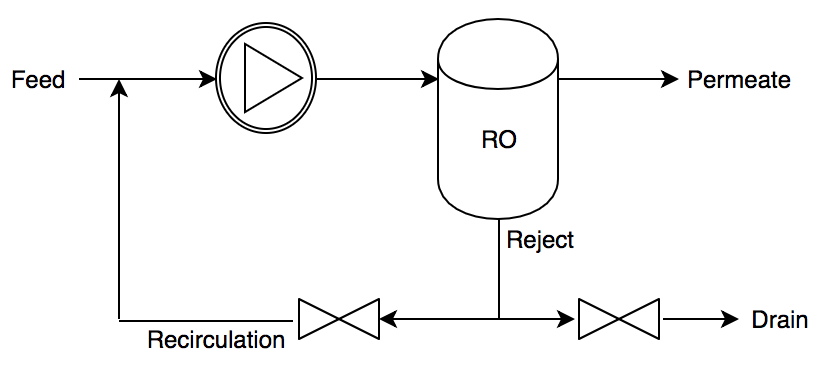
\includegraphics[width=0.8\textwidth]{Sys1}
    \caption{One pump system}
    \label{fig:System1}
\end{minipage}%
\begin{minipage}{.5\textwidth}
  \centering
  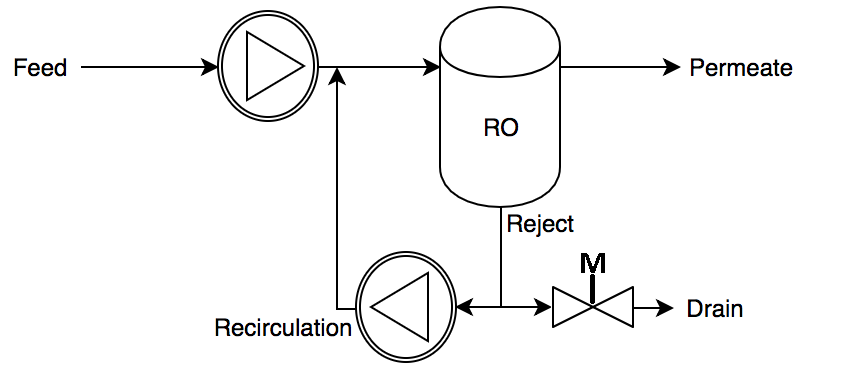
\includegraphics[width=.8\linewidth]{Sys2}
  \caption{Two pump system}
  \label{fig:System2}
\end{minipage}
\end{figure}

\newpage

\section{Investigation}

In order to compare the two systems and understand how the membrane performed in different working conditions both systems needed to be tested. The tests were conducted by controlling the temperature, pumps and the conductivity in the recirculation loop and log how the different conditions affected the system and the membrane. 

The tests were conducted by changing the temperature, recirculation conductivity and pump speed and meassure how the system behaved once it had reached steady state. The tests were divided into three test sequences. One test sequence was performed with room temperatured water (19 C), one with water heated to 30 C and in the last test sequence the water was heated to 40 C. Every test sequence included data from 8 steady state points with different settings on feed conductivity and pump speed. The test sequences are displayed in the table below. 

\begin{table}[H]
\centering
\begin{tabular}{|p{1.4cm}||p{2cm}|p{3.2cm}|p{1.8cm}|}
 \hline
 \textbf{Steady state }&Temperature&Feed Conductivity&Motor effect \\
 \hline
 1.1 & 18 $^\circ$C   & 280 \SI{}{\micro\siemens} & 60 \% \\
 1.2   &  18 $^\circ$C   & 500 \SI{}{\micro\siemens} & 60 \% \\
 1.3 &  18 $^\circ$C  &1000 \SI{}{\micro\siemens} & 60 \% \\
 1.4 &  18 $^\circ$C  &1000 \SI{}{\micro\siemens} & \textbf{80 \%} \\
 1.5 &18 $^\circ$C &2000 \SI{}{\micro\siemens}& 60 \%\\
 1.6 &18 $^\circ$C  &2000 \SI{}{\micro\siemens}& \textbf{80 \%}\\
 1.7   &18 $^\circ$C & 3000 \SI{}{\micro\siemens}&60 \% \\
 1.8   &18 $^\circ$C&3000 \SI{}{\micro\siemens}& \textbf{80 \%}\\
 \hline
 2.1 & 30 $^\circ$C & 280 \SI{}{\micro\siemens}&60 \%\\
 2.2 & 30 $^\circ$C &500 \SI{}{\micro\siemens}& 60 \%\\
 2.3 & 30 $^\circ$C&1000 \SI{}{\micro\siemens}& 60 \%\\
 2.4 & 30 $^\circ$C&1000 \SI{}{\micro\siemens}& \textbf{80 \%}\\
 2.5 & 30 $^\circ$C&2000 \SI{}{\micro\siemens}& 60 \%\\
 2.6 & 30 $^\circ$C&2000 \SI{}{\micro\siemens}& \textbf{80 \%}\\
 2.7 & 30 $^\circ$C& 3000 \SI{}{\micro\siemens}&60 \%\\
 2.8 & 30 $^\circ$C& 3000 \SI{}{\micro\siemens}&\textbf{80 \%}\\
 \hline 
 3.1 & 40 $^\circ$C& 280 \SI{}{\micro\siemens}& 60 \%\\
 3.2 & 40 $^\circ$C &500 \SI{}{\micro\siemens}& 60 \%\\
 3.3 & 40 $^\circ$C  & 1000 \SI{}{\micro\siemens}& 60 \%\\
 3.4 & 40 $^\circ$C  & 1000 \SI{}{\micro\siemens}& \textbf{80 \%}\\
 3.5 & 40 $^\circ$C&2000 \SI{}{\micro\siemens}& 60 \%\\
 3.6 & 40 $^\circ$C &2000 \SI{}{\micro\siemens}& \textbf{80 \%}\\
 3.7 & 40$^\circ$C &3000 \SI{}{\micro\siemens}& 60 \%\\
 3.8 & 40$^\circ$C &3000 \SI{}{\micro\siemens}& \textbf{80 \%}\\
\hline
\end{tabular}
\caption{Testcases}
    \label{tab:test cases} 
\end{table}


\subsection{Current system, Test sequence 1, part 1}

The water in the tank was heated while the test was running. Because of this, the test was split up in two parts, first the motor was set to 60\% and steady state 1.1, 1.2, 1.3, 1.5 and 1.7 were investigated. In the part 2, the motor was set to 80 \% and steady state 1.4, 1.6 and 1.8 were investigated. 
\begin{figure}[H]
    \centering
    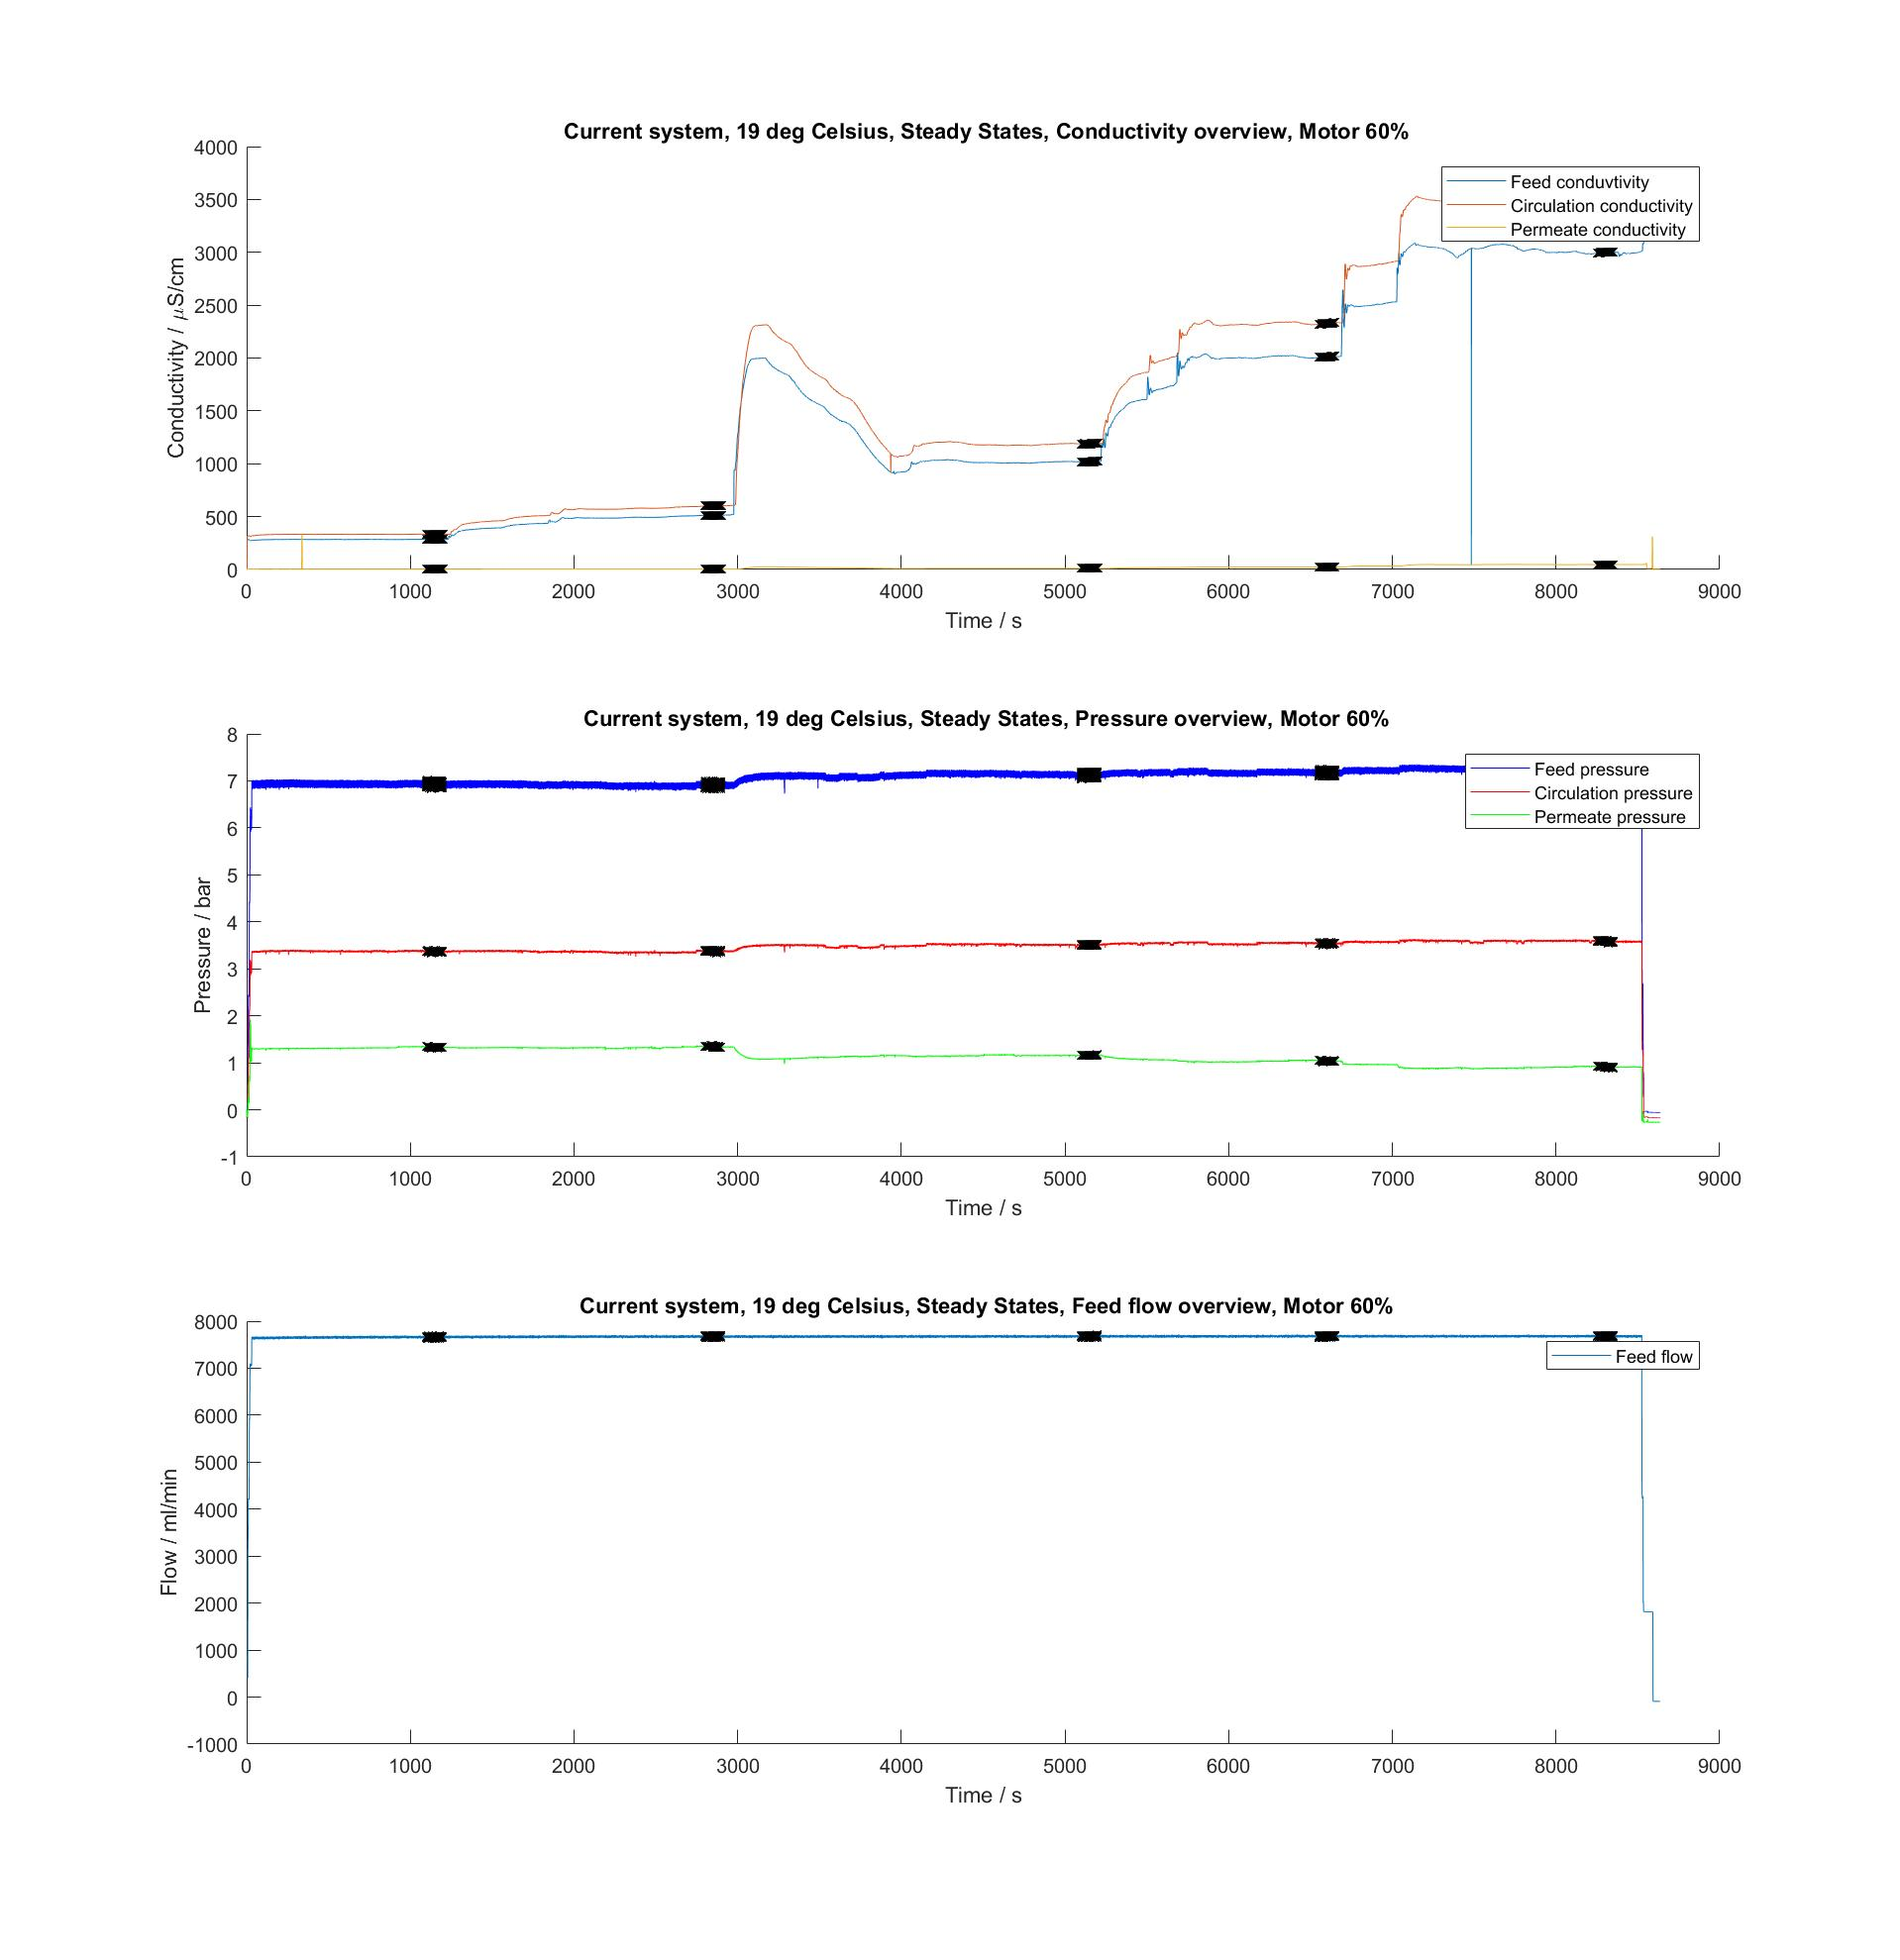
\includegraphics[width=1.1\textwidth]{overview20_60}
    \caption{Test 1, Current system, 18 degrees celsius. Steady states 1.1, 1.2, 1.3, 1.5 and 1.7 }
    \label{fig:PressConn}
\end{figure}

\newpage

\subsection{Current system, Test sequence 1, part 2}
  
\begin{figure}[H]
    \centering
    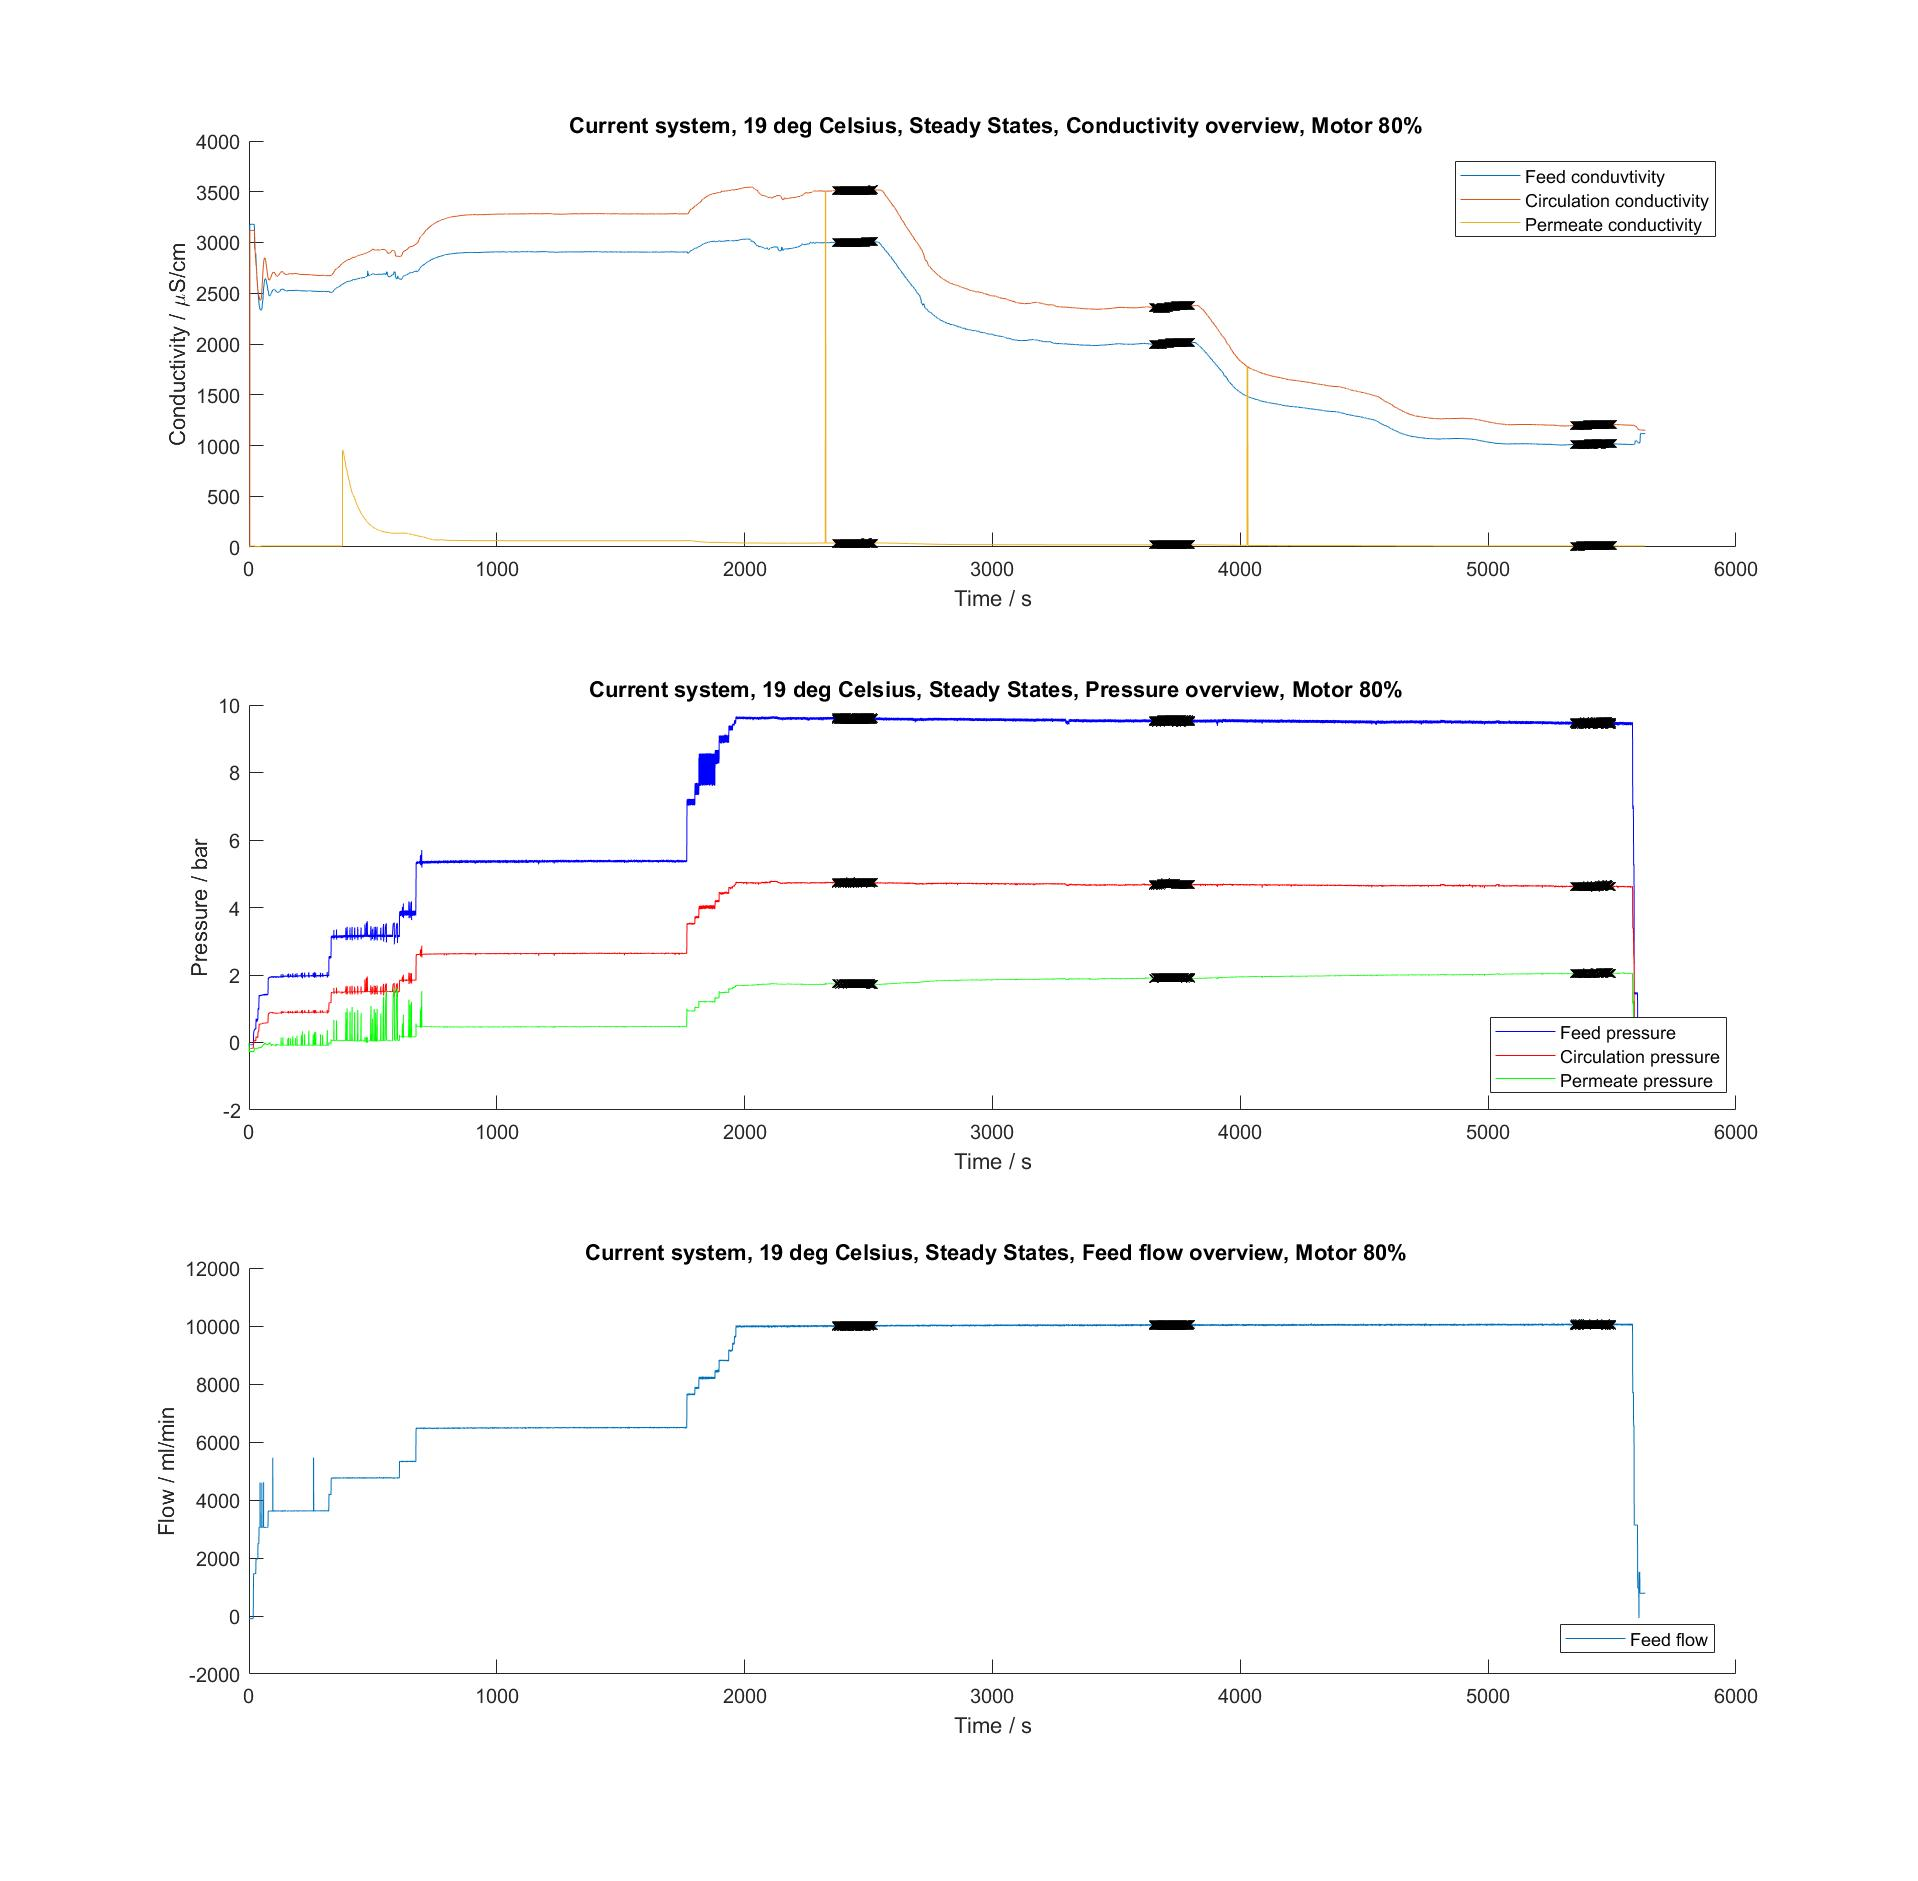
\includegraphics[width=1.1\textwidth]{overview20_80}
    \caption{Test 1, Current system, 18 degrees celsius. Steady states 1.4, 1.6 and 1.8}
    \label{fig:PressConn}
\end{figure}

\newpage

By post-procesing the data from test one in Matlab it was possible to visually show how the system parameters were affected by the changed pump speed and feed conductivity. 


insert table, results on how the different graphs changed!!!

\begin{figure}[H]
    \centering
    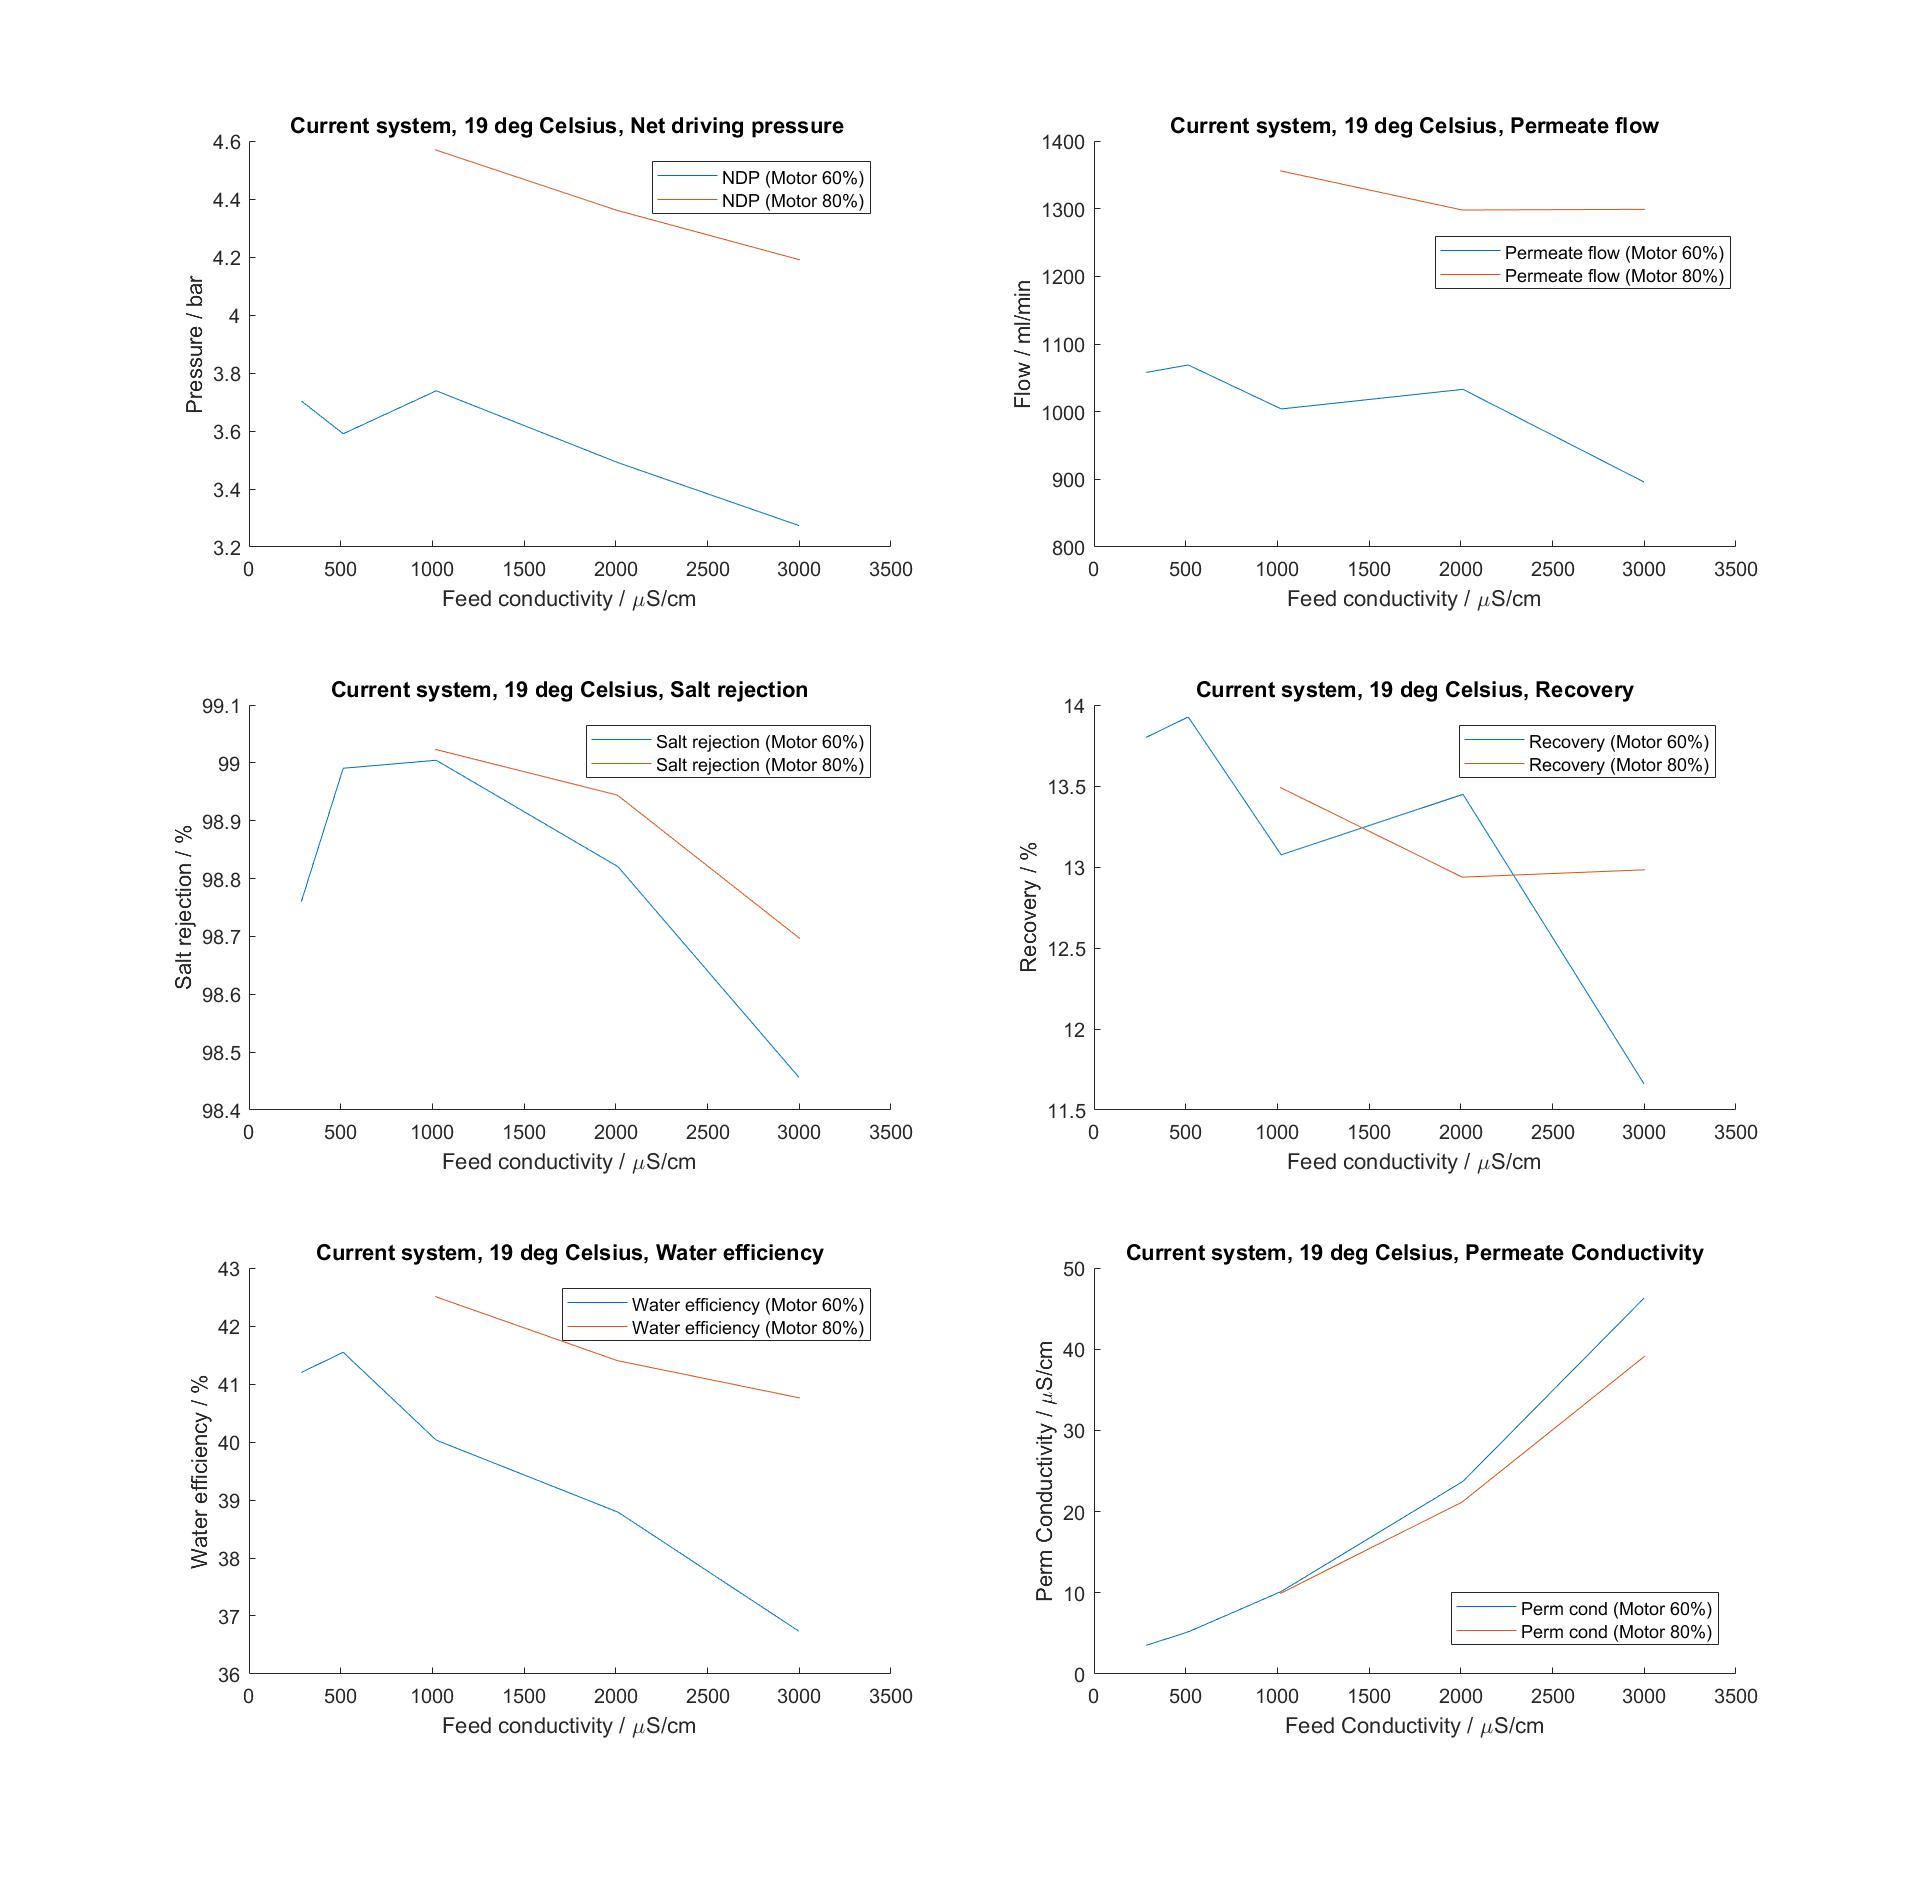
\includegraphics[width=1.1\textwidth]{Key20}
    \caption{Connections Pressure sensors}
    \label{fig:PressConn}
\end{figure}

\newpage

\subsection{Current system, Test sequence 2}

The second test was carried out by setting the heater bath to 30 degrees celsius and and adjusting the conductivity and pump speed according to the test plan. Since the water was much warmer than the air in the room, the heating caused by the pump was not as prominent and allowed all steady states to be examined in one contimous test.

\begin{figure}[H]
    \centering
    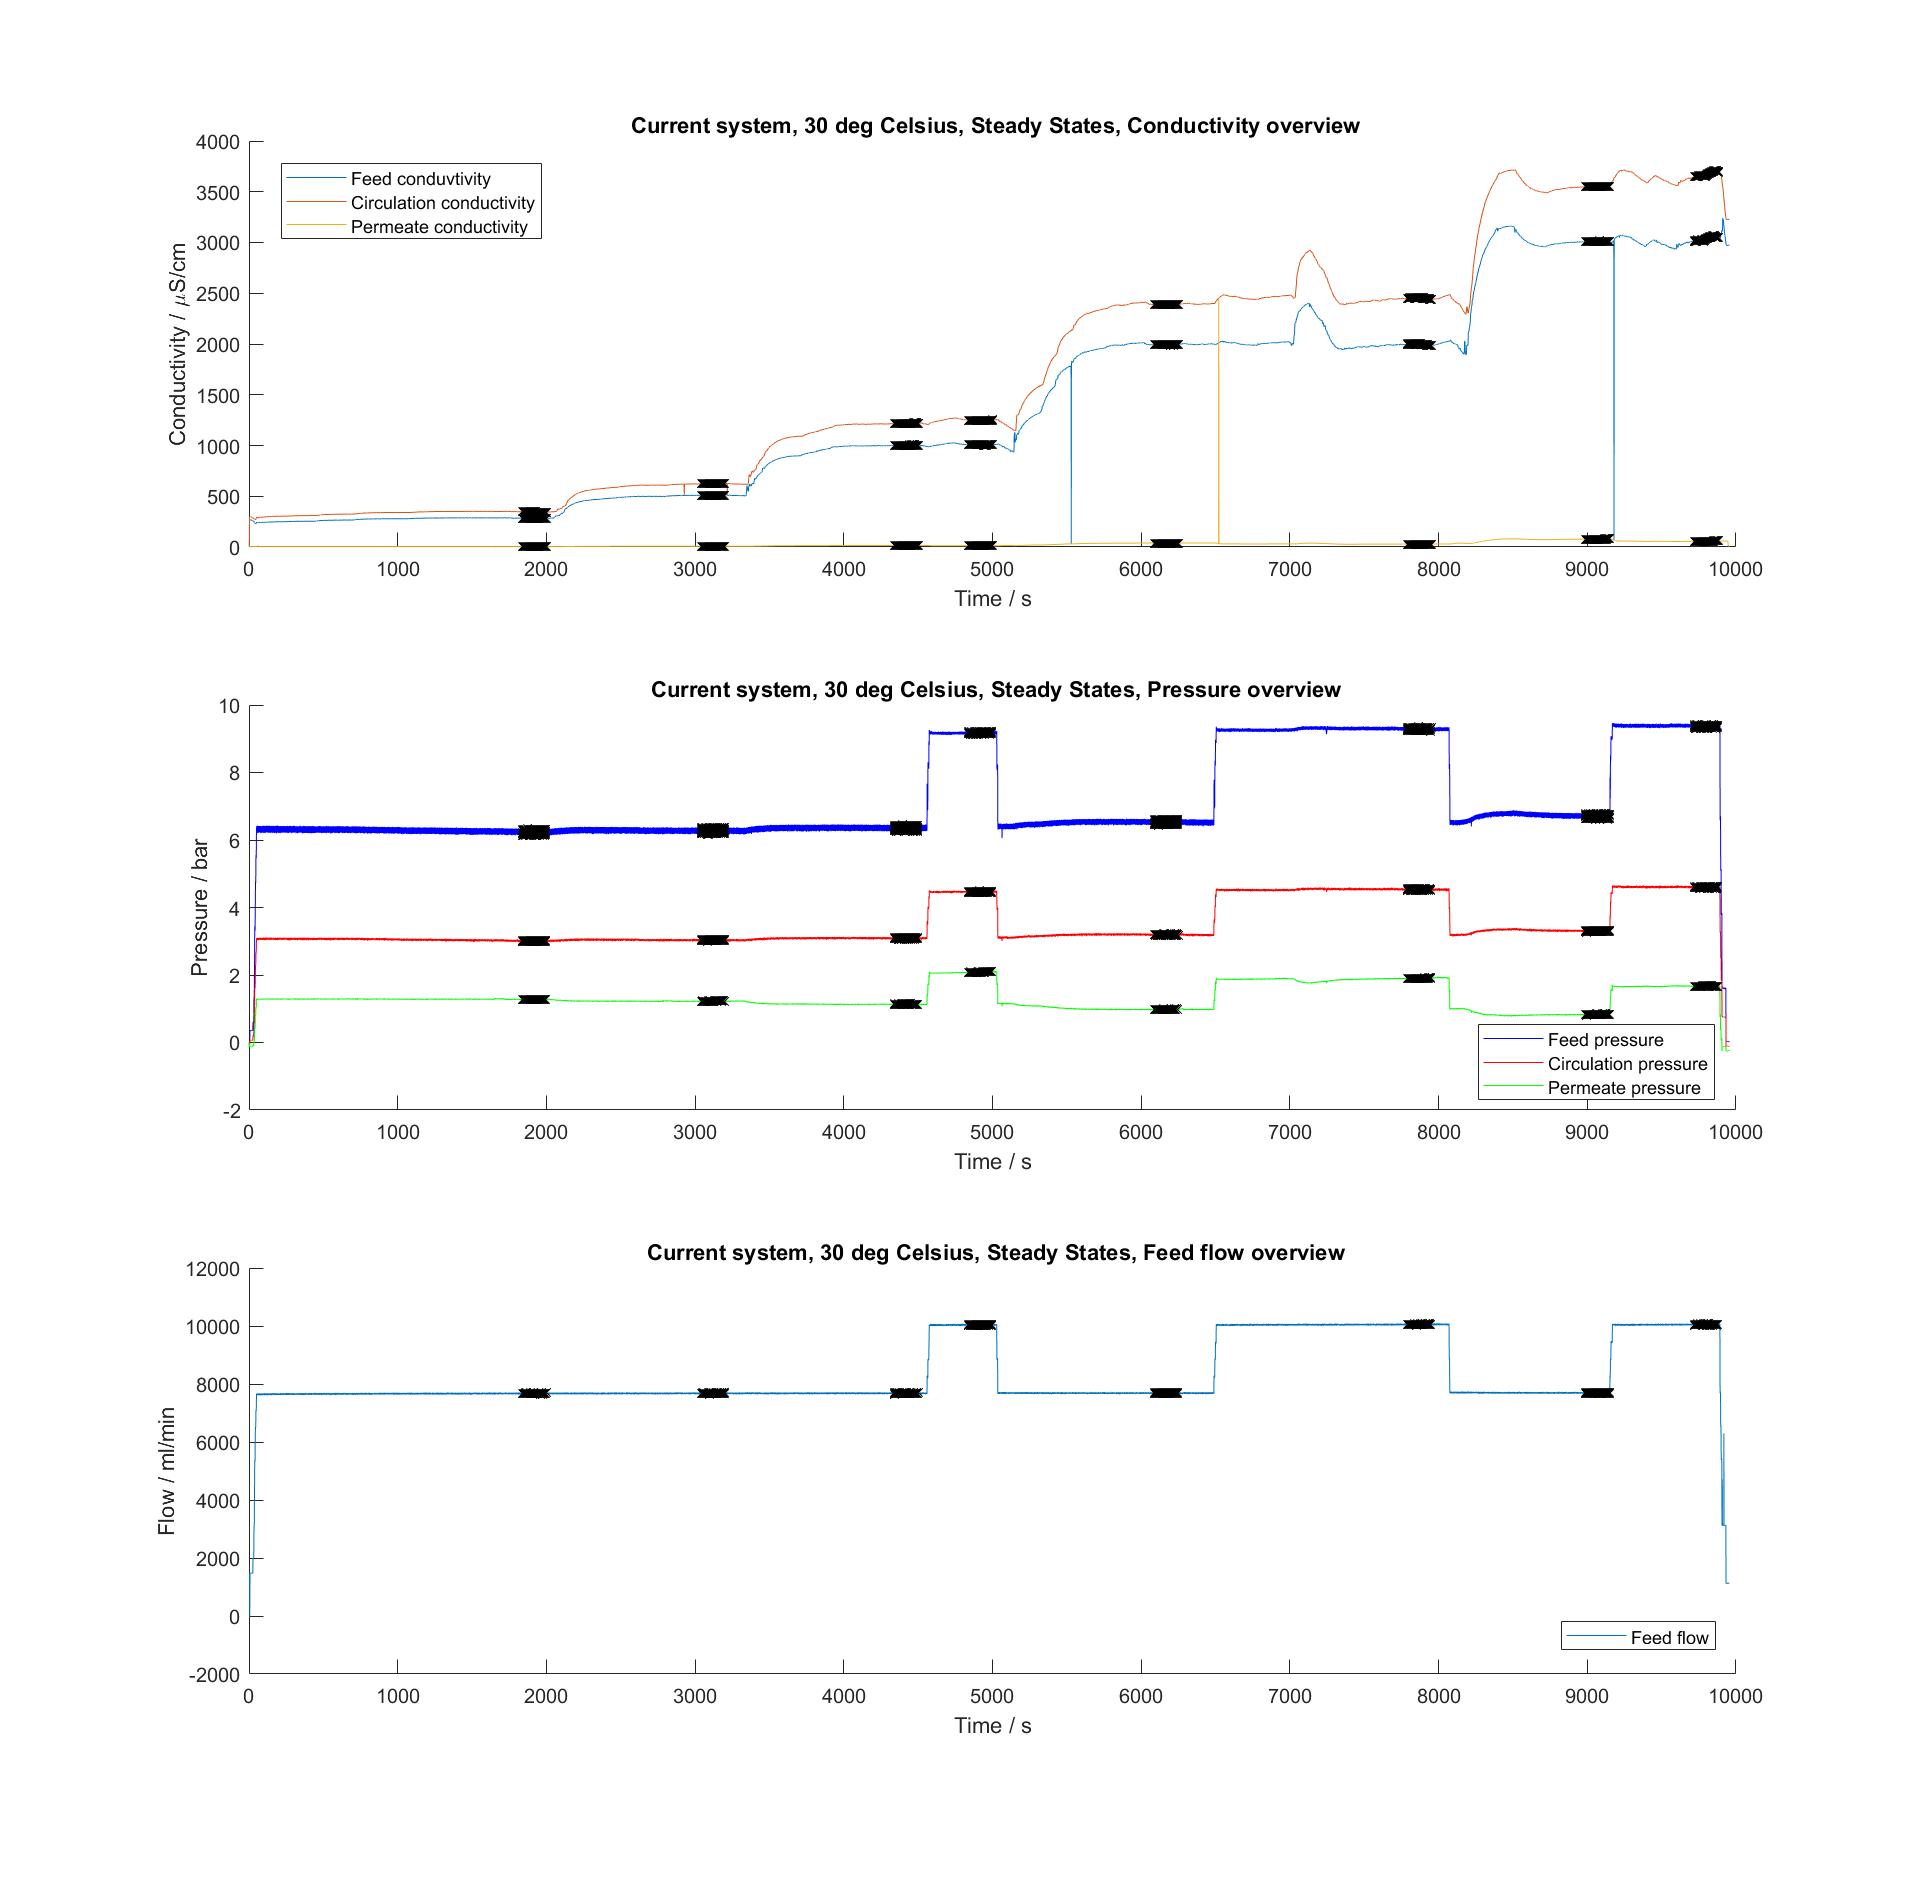
\includegraphics[width=1.1\textwidth]{overview30}
    \caption{Test 2, Current system, 30 degrees celsius. Steady states 1.1, 1.2, 1.3, 1.4 1.5, 1.6, 1.7 and 1.8}
    \label{fig:PressConn}
\end{figure}

\newpage



The data from the test was post proccesed in Matlab in exactly the same way as the previous test.

\begin{figure}[H]
    \centering
    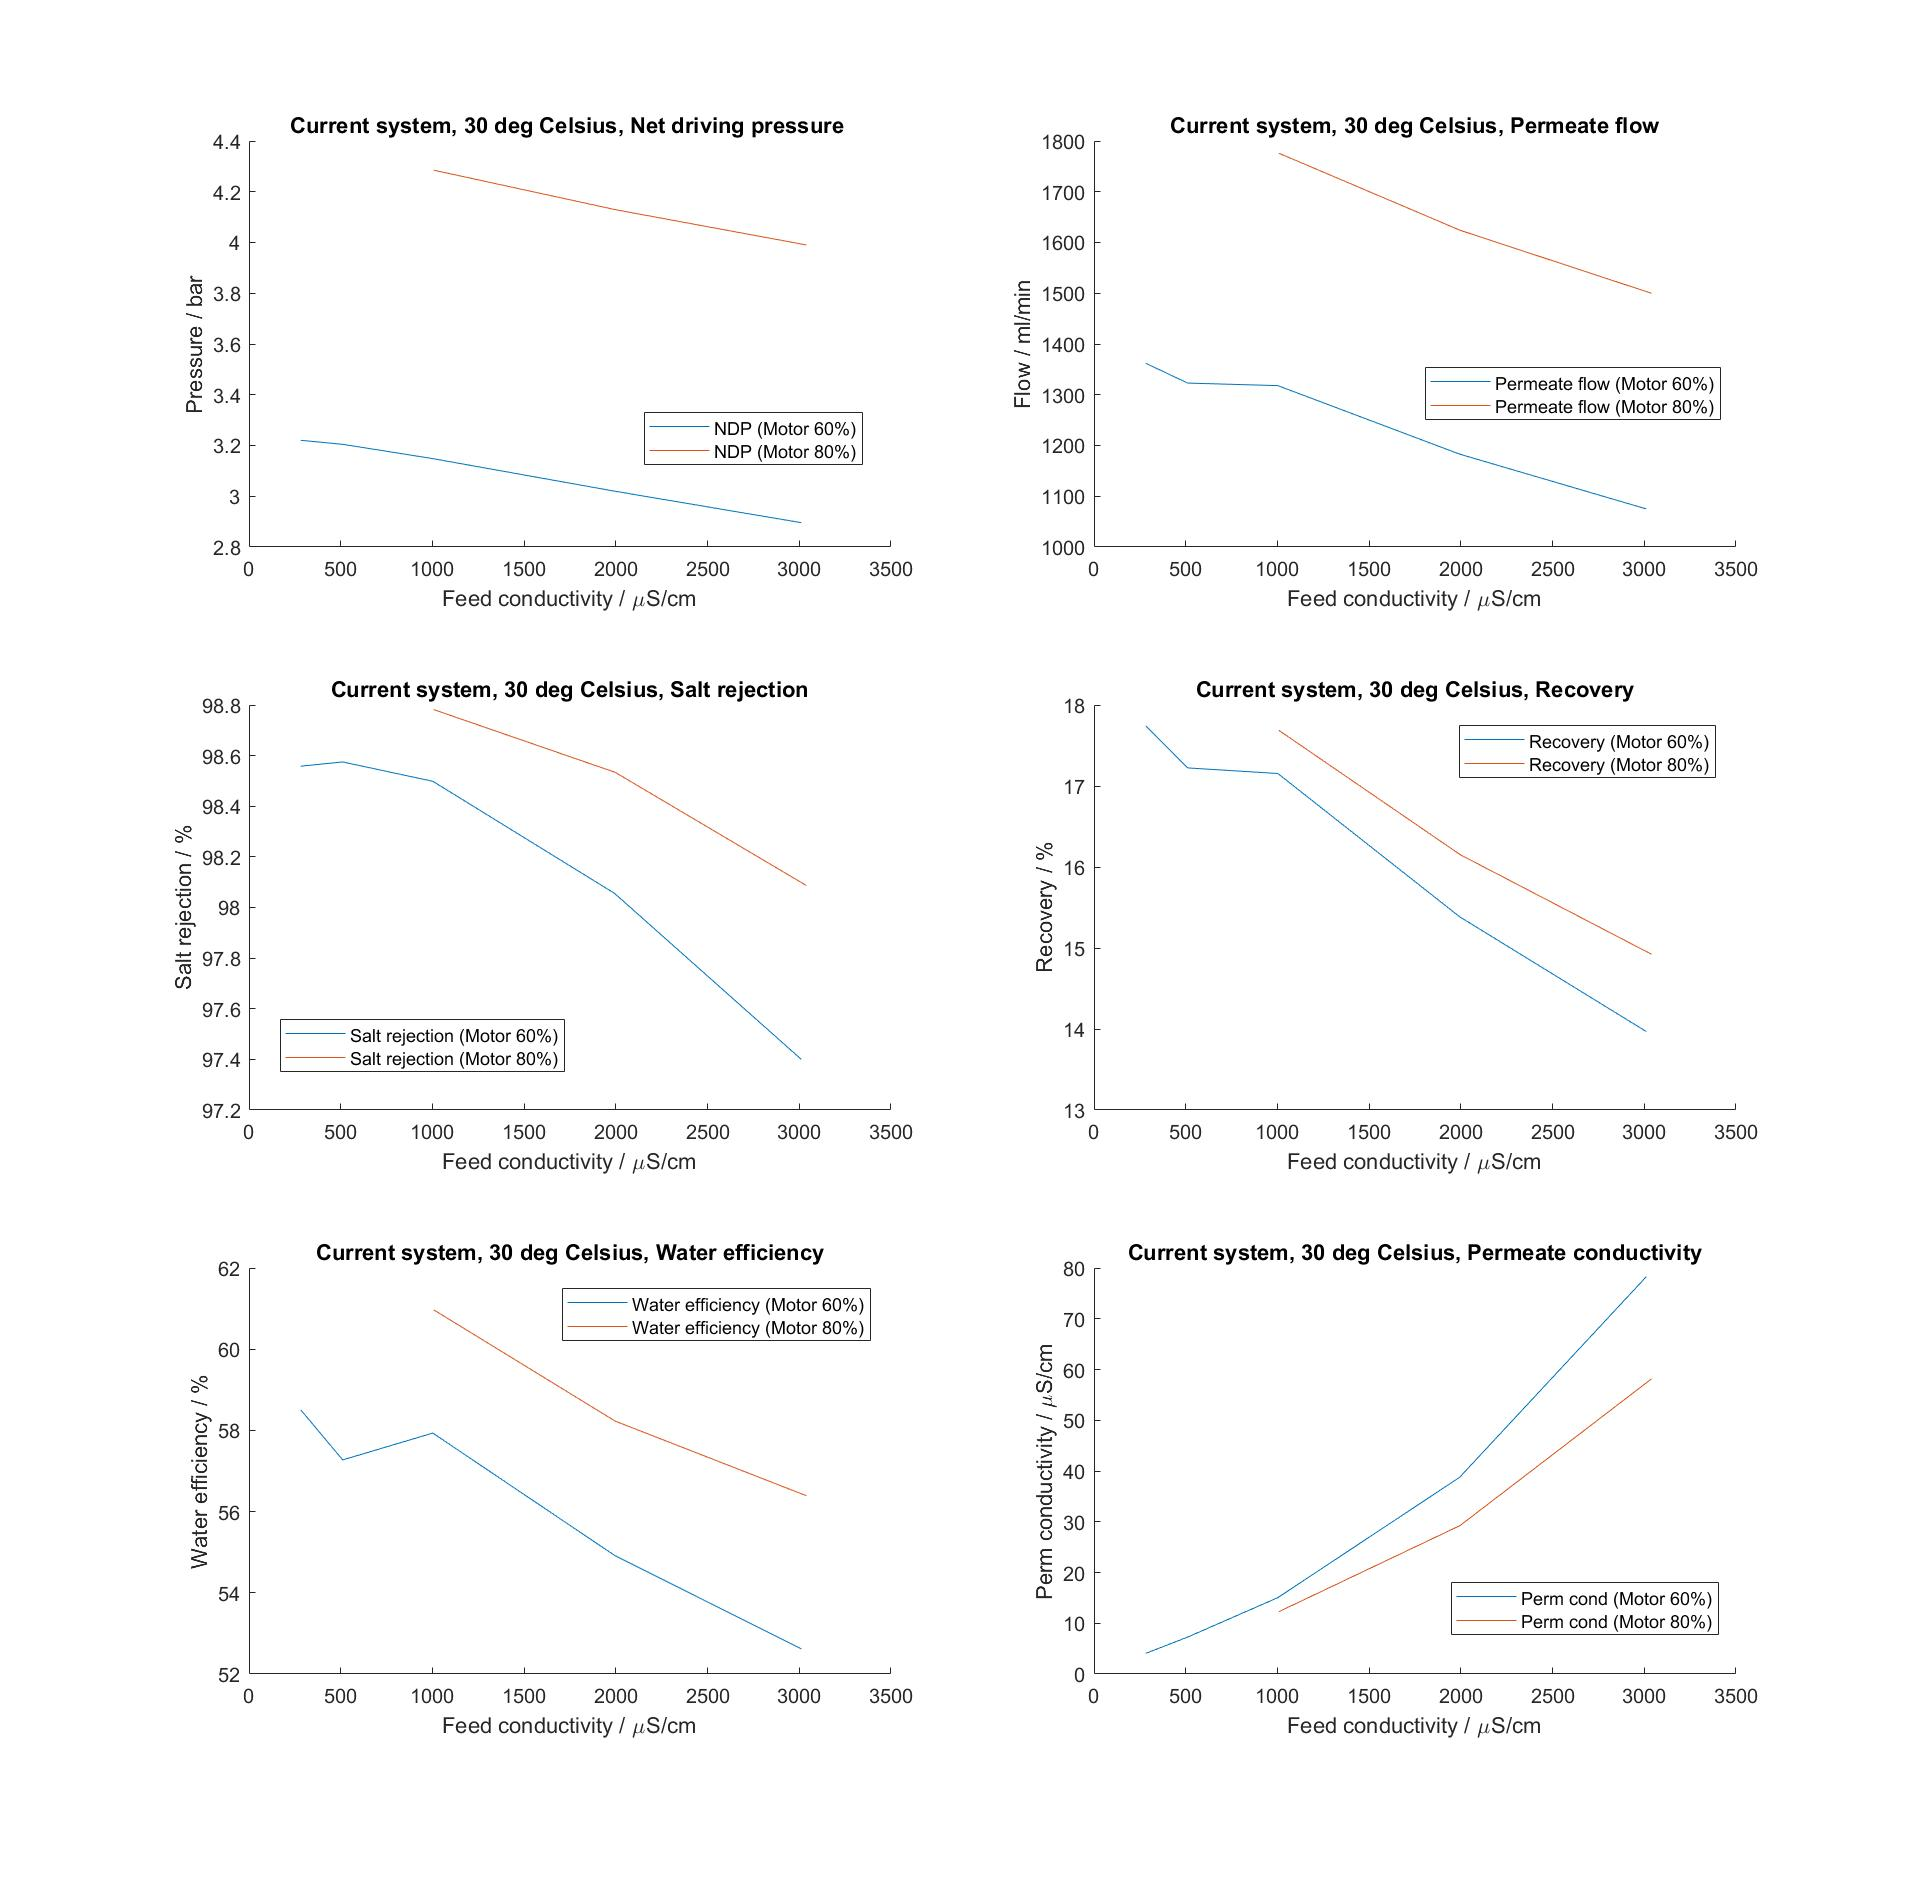
\includegraphics[width=1.1\textwidth]{Key30}
    \caption{Connections Pressure sensors}
    \label{fig:PressConn}
\end{figure}

\newpage

\subsection{Current system, Test sequence 3}

Finally the heating bath was set to 40 C and the test sequence was performed just like test sequence 2. 

\begin{figure}[H]
    \centering
    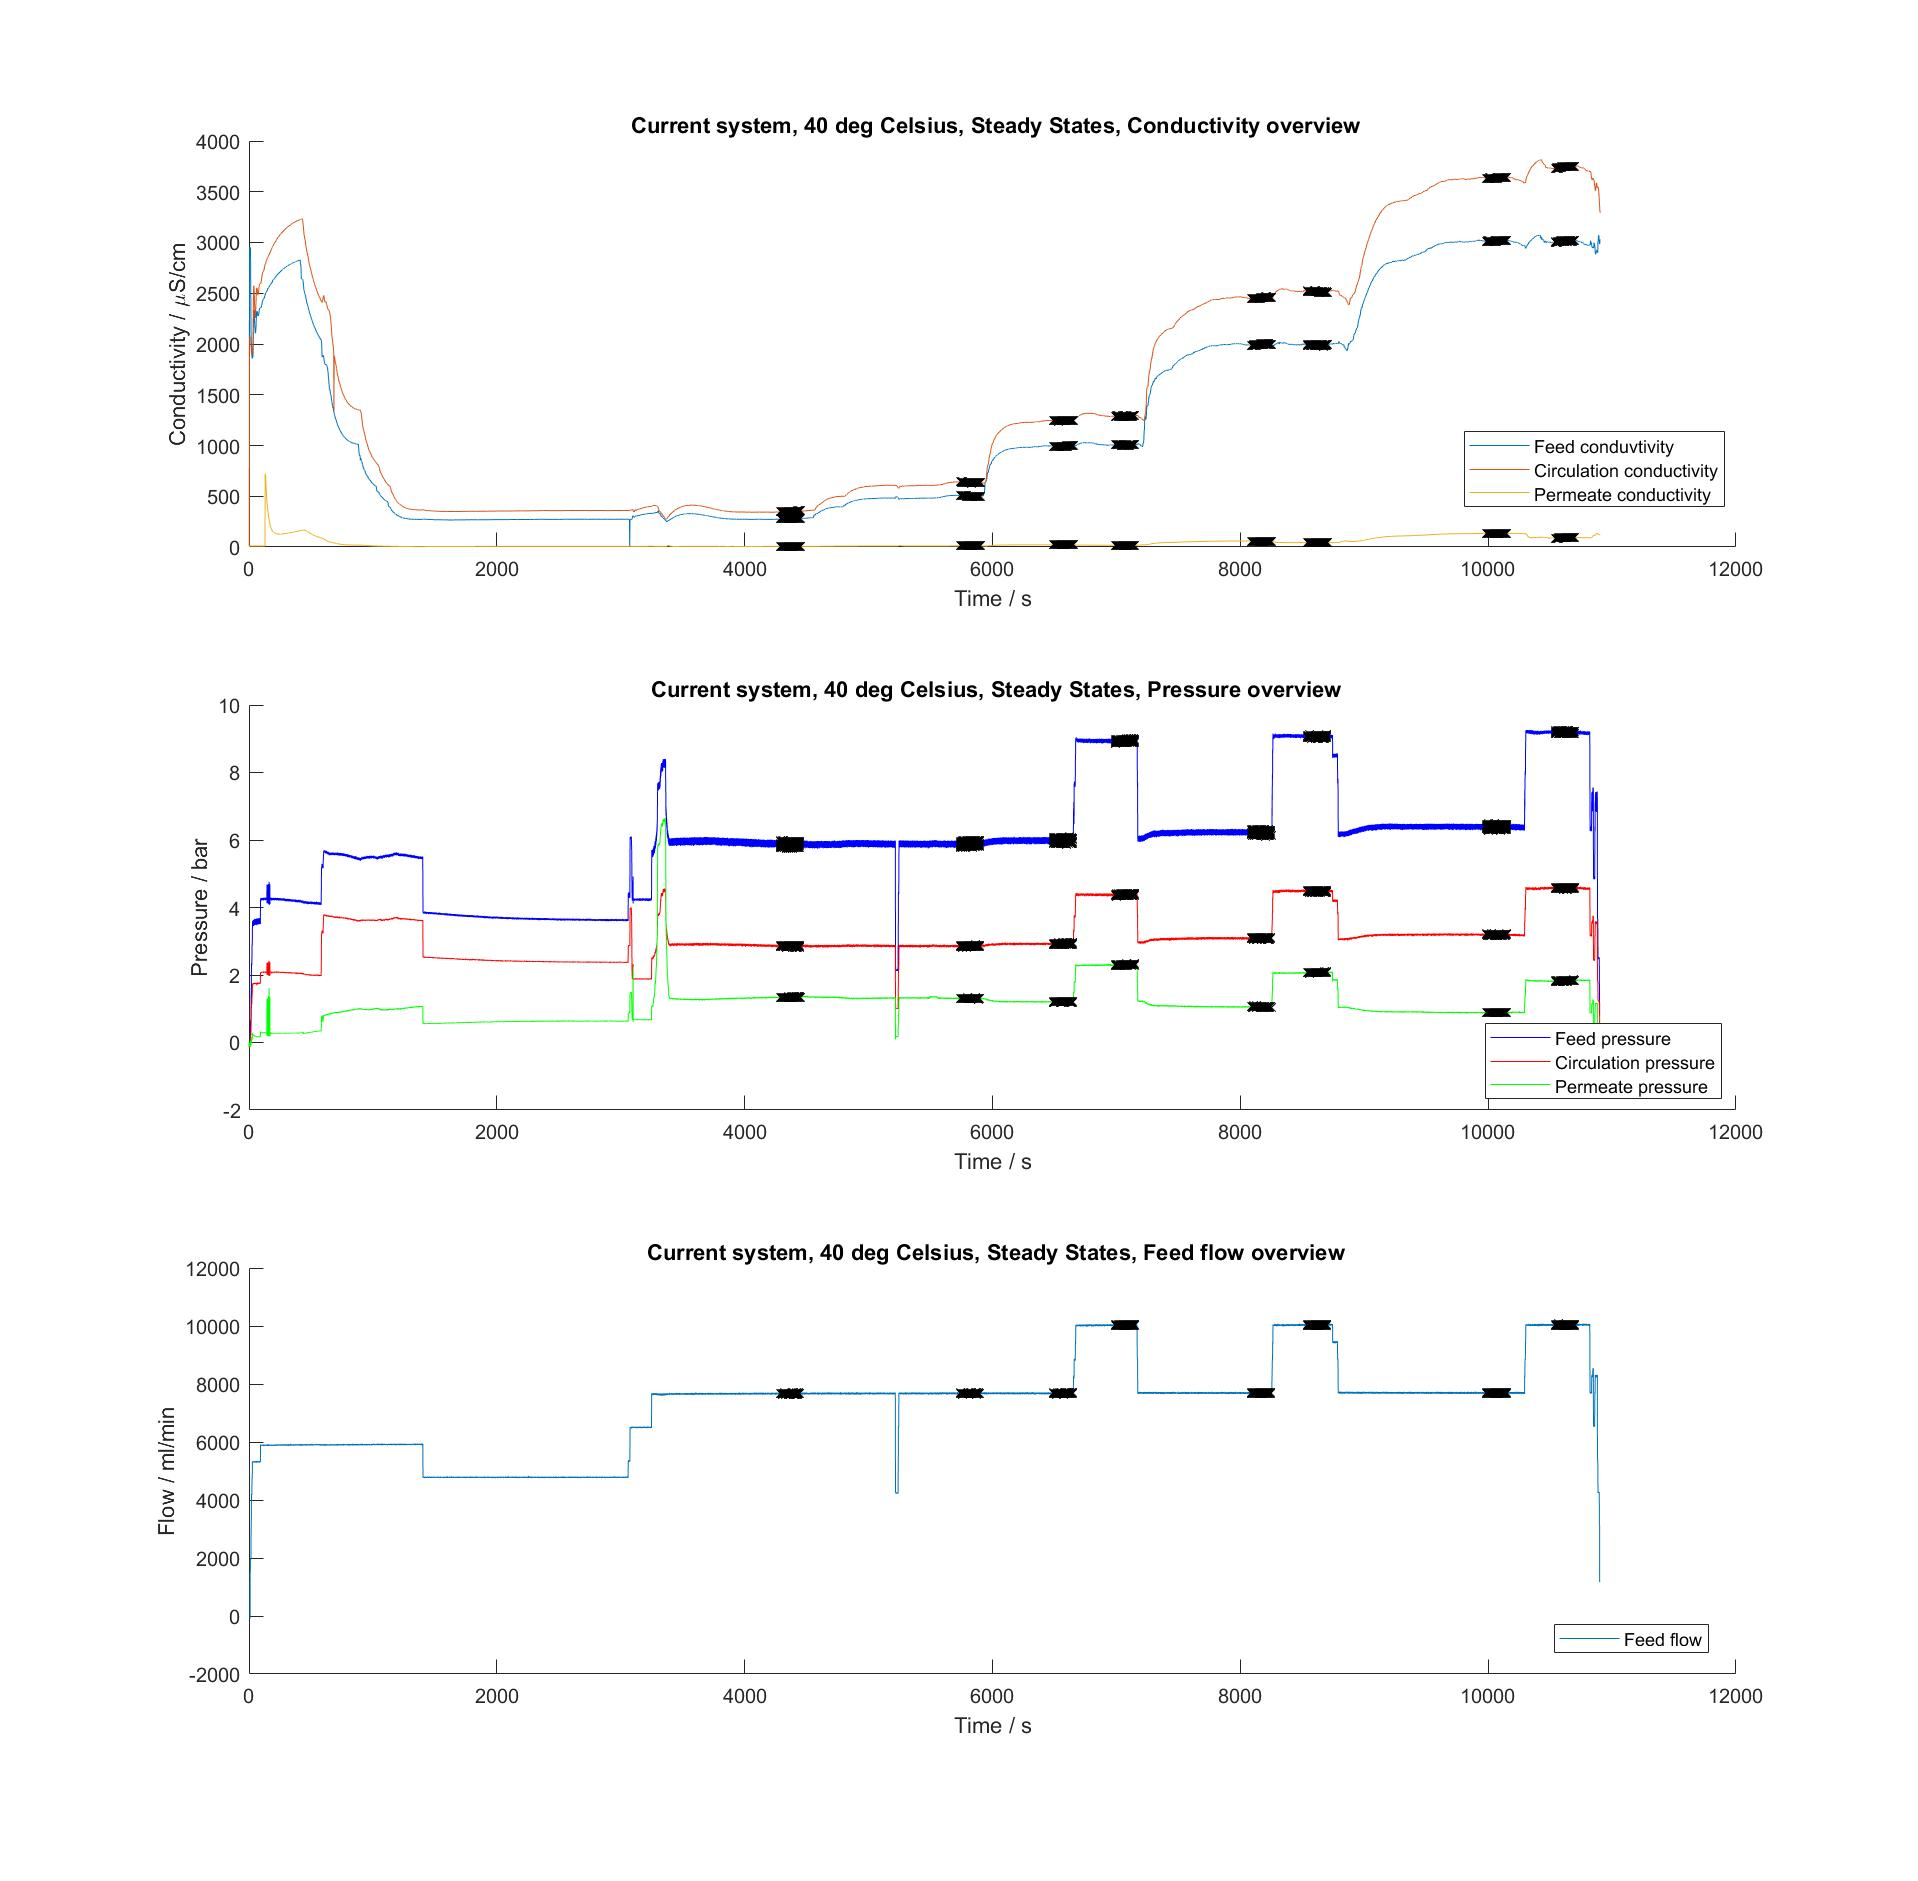
\includegraphics[width=1.1\textwidth]{overview40}
    \caption{Connections Pressure sensors}
    \label{fig:PressConn}
\end{figure}

\newpage

Post processing in matlab generated the following data from the steady states.

\begin{figure}[H]
    \centering
    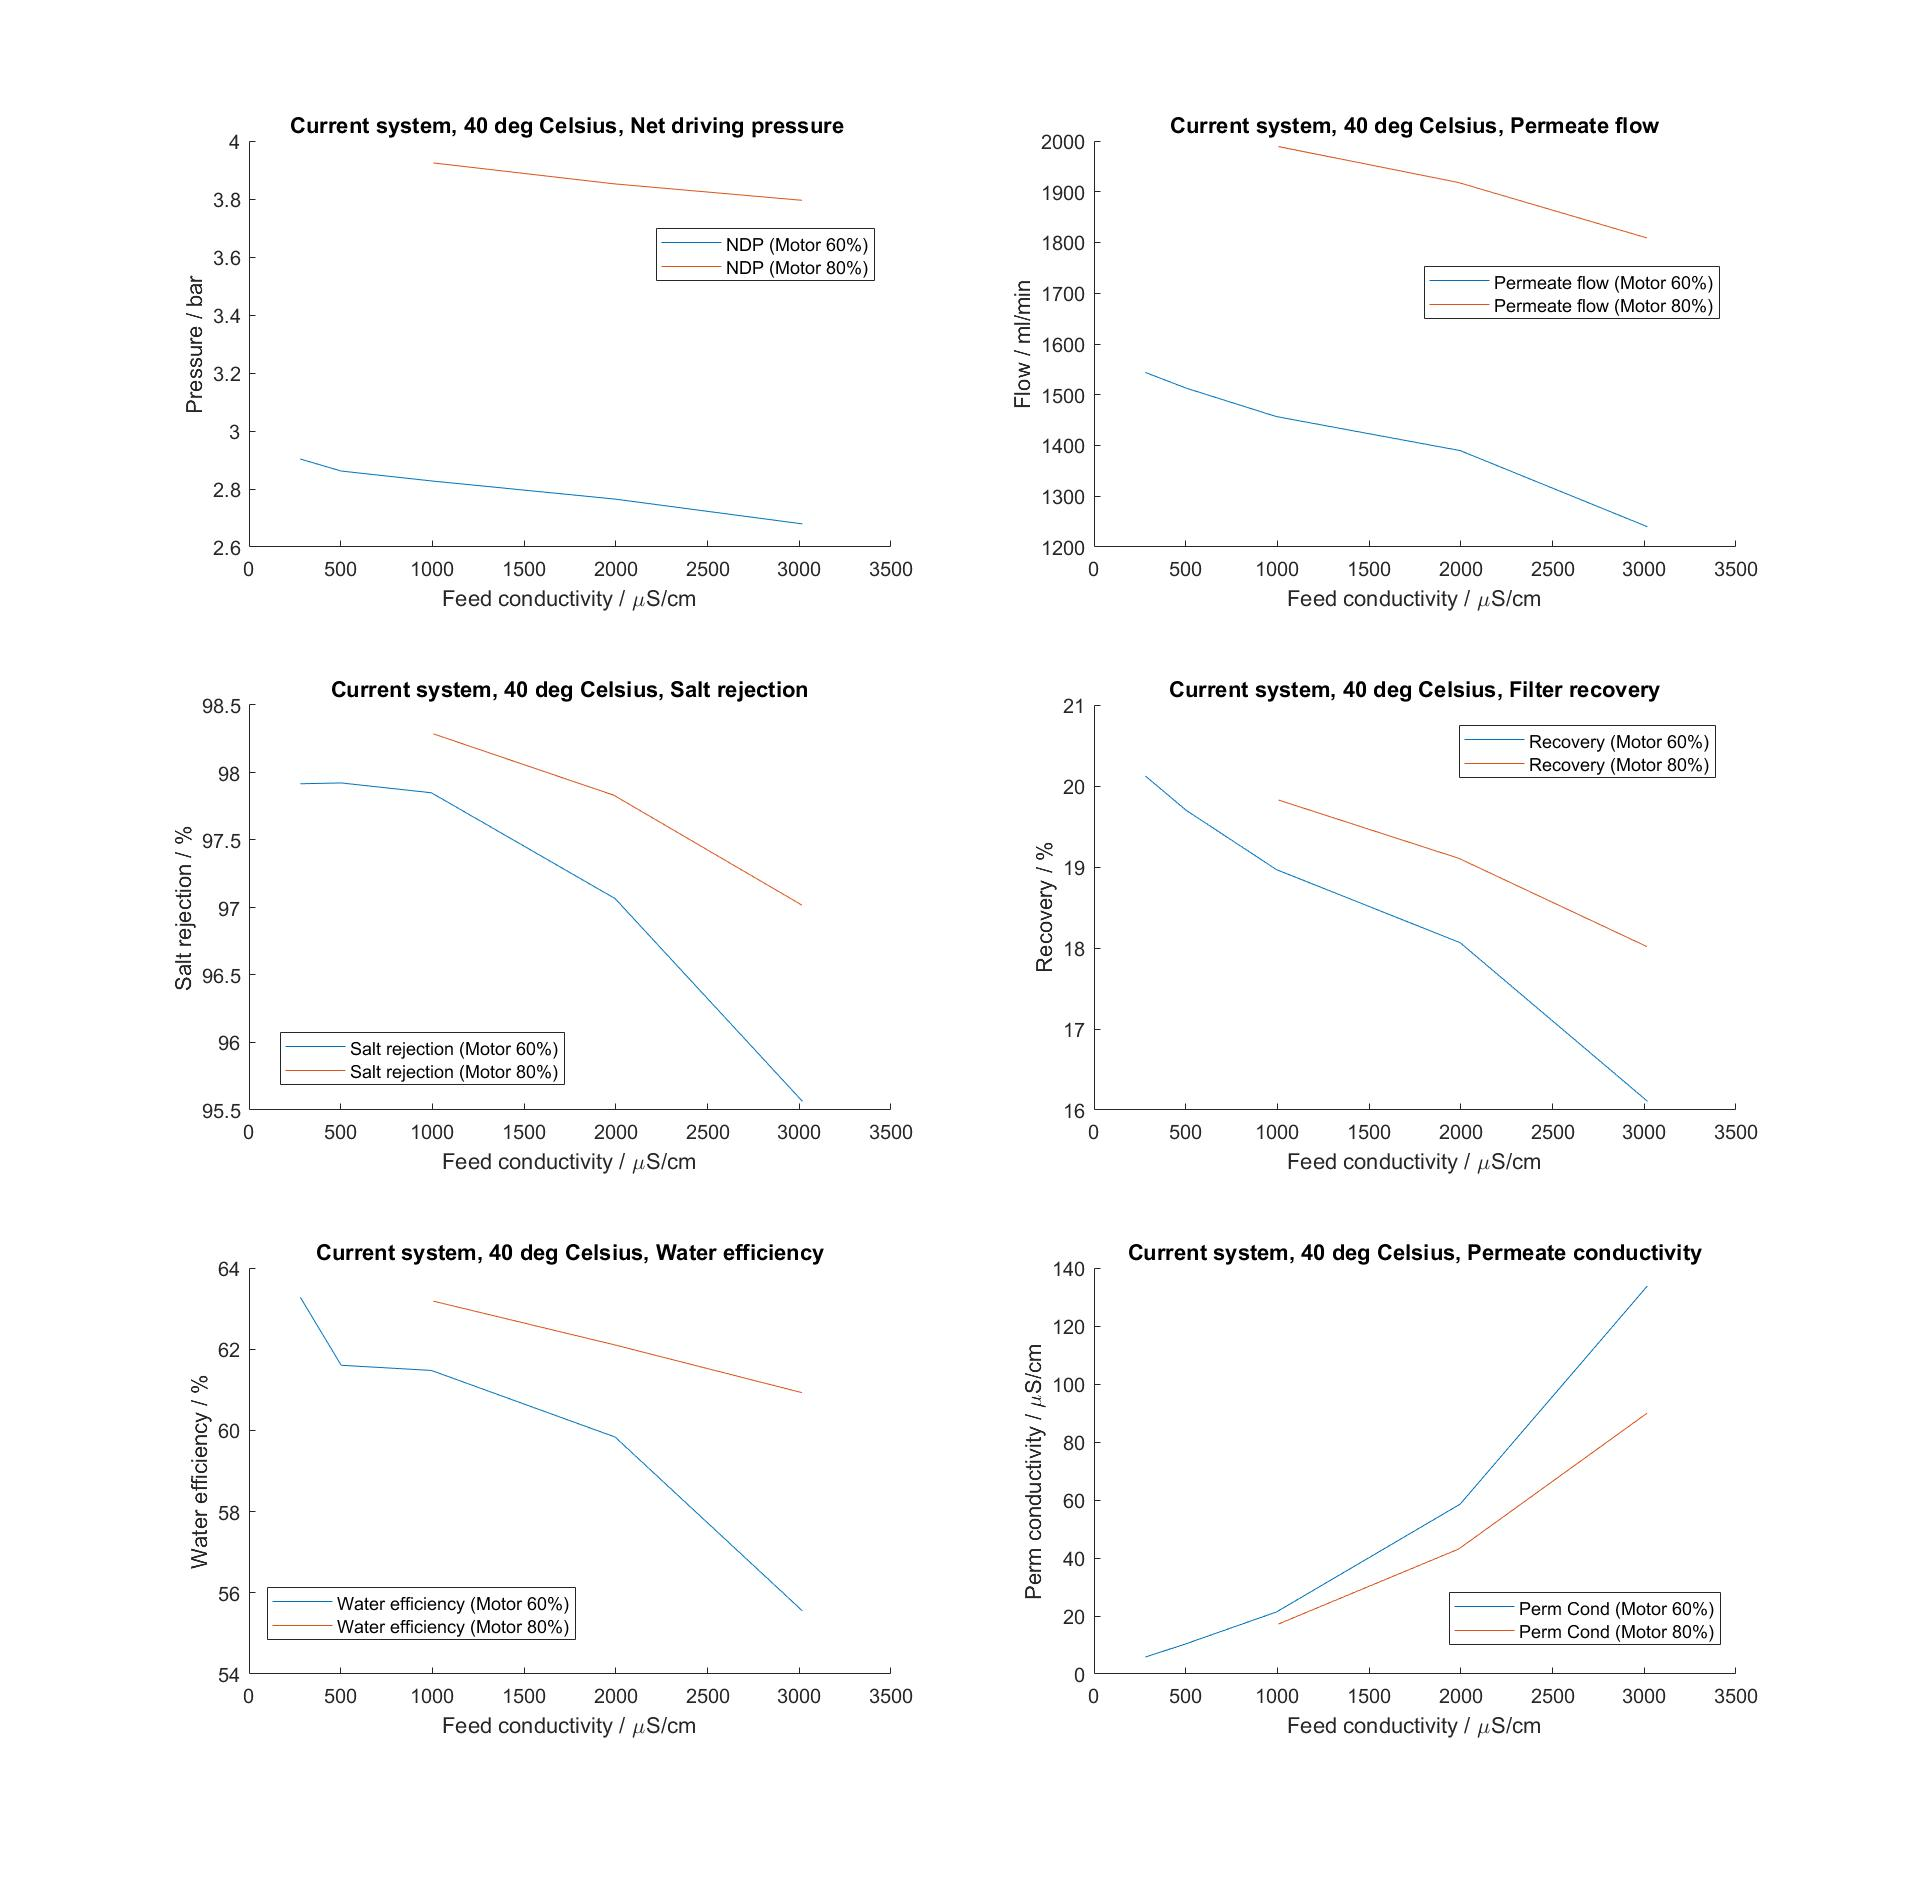
\includegraphics[width=1.1\textwidth]{Key40}
    \caption{Connections Pressure sensors}
    \label{fig:PressConn}
\end{figure}

\newpage

In order to understand how the system current performed in different working conditions all plots from the post processing in Matlab was put togheter. 

\subsection{Net driving pressure}

Net driving pressure was decreased when the temperature was increased. Higher feed conductivity resulted in a decreased net driving pressure. As expected, running the feed pump at a higher RPM also increased the net driving pressure.

\begin{figure}[H]
    \centering
    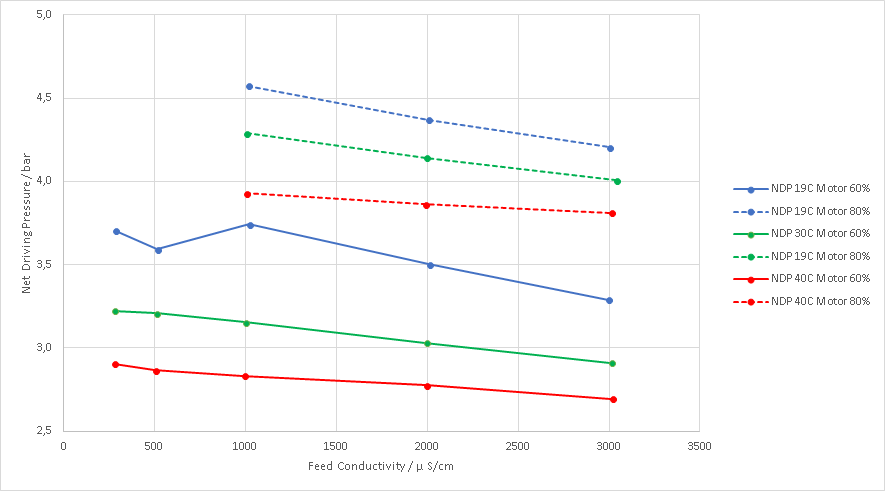
\includegraphics[width=0.8\textwidth]{NDP}
    \caption{Net driving pressure}
    \label{fig:PressConn}
\end{figure}

\subsection{Permeate flow}

According to theory, Net driving pressure has a direct effect on permeate flow. When the feed pump was increased more water was pushed through the membrane. Increased water temperatures caused a much higher permeate flow. For instance, the permeate flow increased by around 50\% when the temperature was increased from 19 C to 40 C and the pump was running at 60\%. Due to the increased osmotic pressure, permeate flow decreased when the feed conductivity increased

\begin{figure}[H]
    \centering
    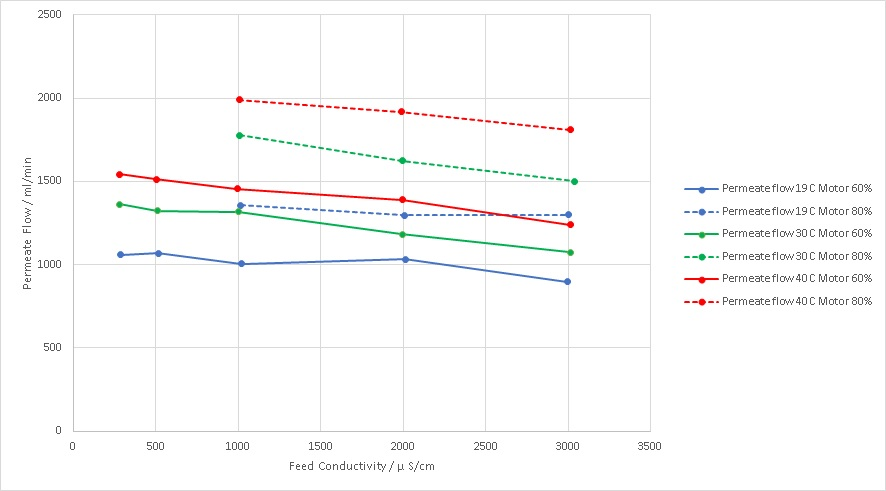
\includegraphics[width=0.8\textwidth]{permFlowCurrent}
    \caption{Connections Pressure sensors}
    \label{fig:PressConn}
\end{figure}

\subsection{Recovery}

Warmer water enabled more feed water to pass through the membrane and therefore the recovery was increased. Increased conductivity reduced recovery due to the increased osmotic pressure.

\begin{figure}[H]
    \centering
    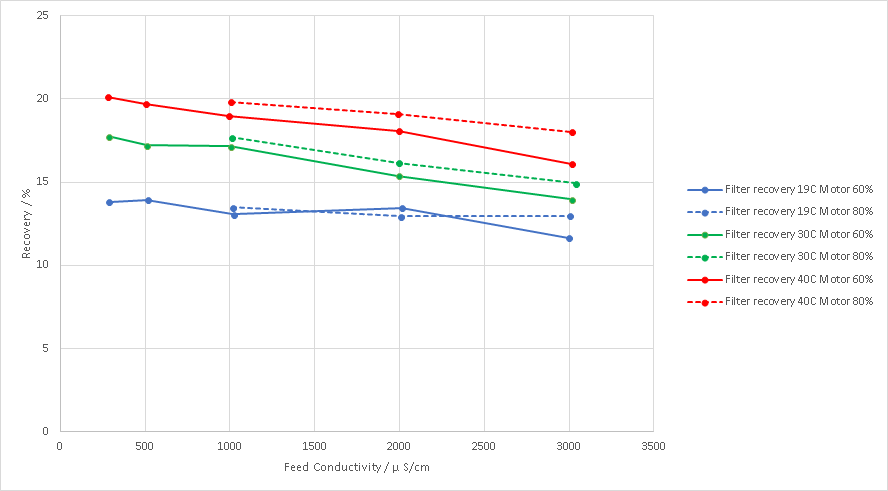
\includegraphics[width=0.8\textwidth]{Recovery}
    \caption{Connections Pressure sensors}
    \label{fig:PressConn}
\end{figure}

\subsection{Salt rejection}

By looking at plot 5.13 the deterimental effects of both increased temperature and feed conductivity can be seen. The negative effect of increased feed conductivity was much more prominent at 40 C than 30C which means that the performance of the membrane decreased exponentially with higher temperature. Increased feed pump pressure resultet in better salt rejection and the positive effect of increased pump pressure was larger when the system was hot. Temperature was the parameter that decreased salt rejetion the most and by comparing how the system performed when the pump and feed conductivity was set to 60\% and 3000uS/cm at 19C and 40C it can be seen that the salt rejection decreased from 98.5\% to 95.5 \%. From the experiment it can also be concluded that the system perform much better at low temperature and feed conductivity that at high temperature and feed conductivity. 

\begin{figure}[H]
    \centering
    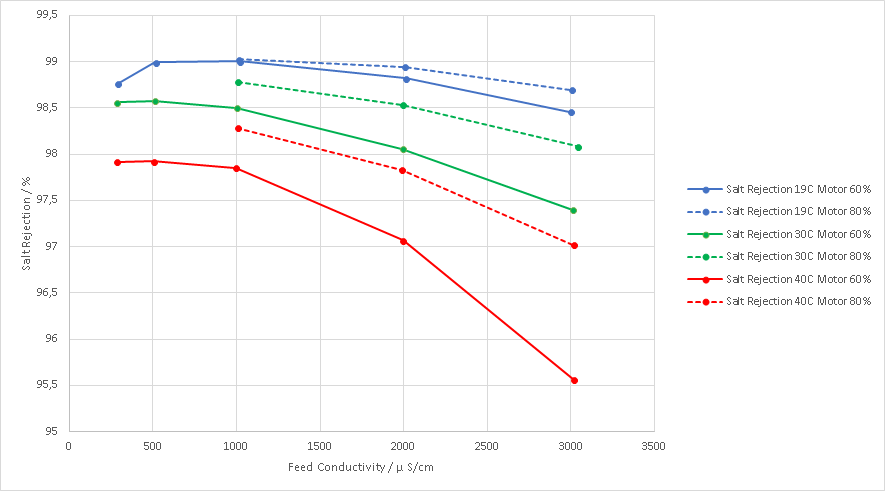
\includegraphics[width=0.8\textwidth]{SaltRejection}
    \caption{Connections Pressure sensors}
    \label{fig:PressConn}
\end{figure}
 
\subsection{Permeate conductivity}

Permeate conductivity was directly proportional to salt rejection at a certain termperature and feed conductivity. The black line in plot 5.14 show the critical permeate conductivity that the system should be able to maintain and from the plot it is possible to se how high the conductivity can be in the recirculation loop without exceeding this limit. The operational area for the different temperature and pump pressure can be seen in plot TBD below.

\begin{figure}[H]
    \centering
    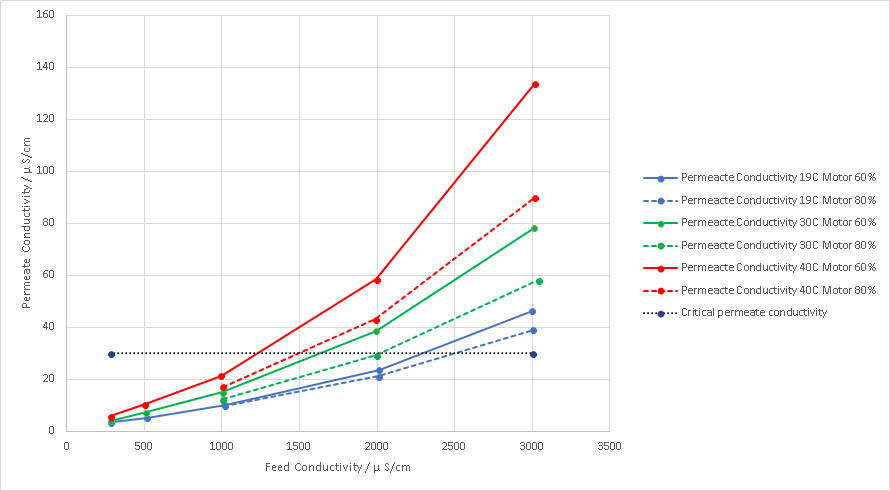
\includegraphics[width=0.8\textwidth]{PermCond}
    \caption{Connections Pressure sensors}
    \label{fig:PressConn}
\end{figure}

!!INSERT TABLE!!

\subsection{Water efficiency}

Water efficiency increased when the temperature increased due to more permeate water being generated by the same feed pressure.

\begin{figure}[H]
    \centering
    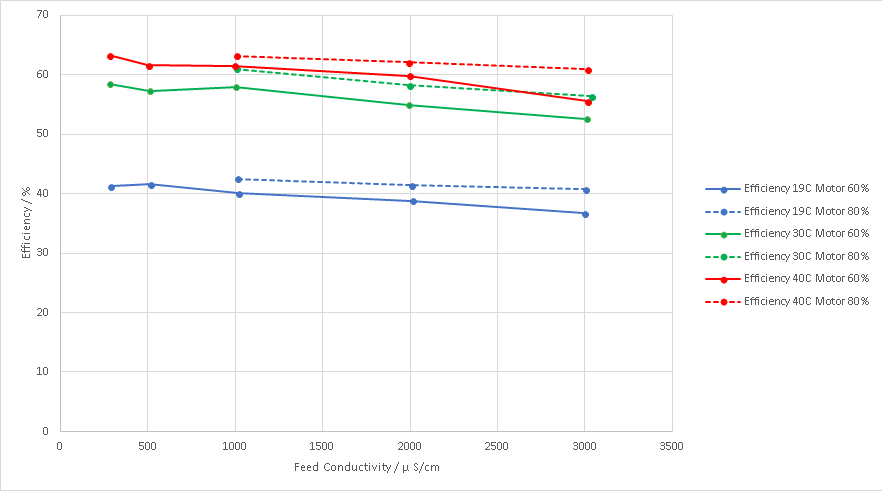
\includegraphics[width=0.8\textwidth]{Efficiency}
    \caption{Connections Pressure sensors}
    \label{fig:PressConn}
\end{figure}

\subsection{System 2}

Test: increaed feed pressure:

Add all plots from test with two pump system. TBD 

Section not finished! 

Kommentar. 

Först lägger vi in plottarna som utvärderar hur de olika parametrarna påverkar systemet med två pumpar.

Därefter kom vi på hur man skulle optimera systemet.

Sen körde vi tester för att hitta en optimal kurva.

Tanken är att presentera resultat, beskriva varför vi valde att optimera systemet på det här sättet och till slut visa hur vi testade oss fram till och beräknade en kurva för att omvända temperatur till en setpoint för permeatflöded.

\begin{figure}[H]
    \centering
    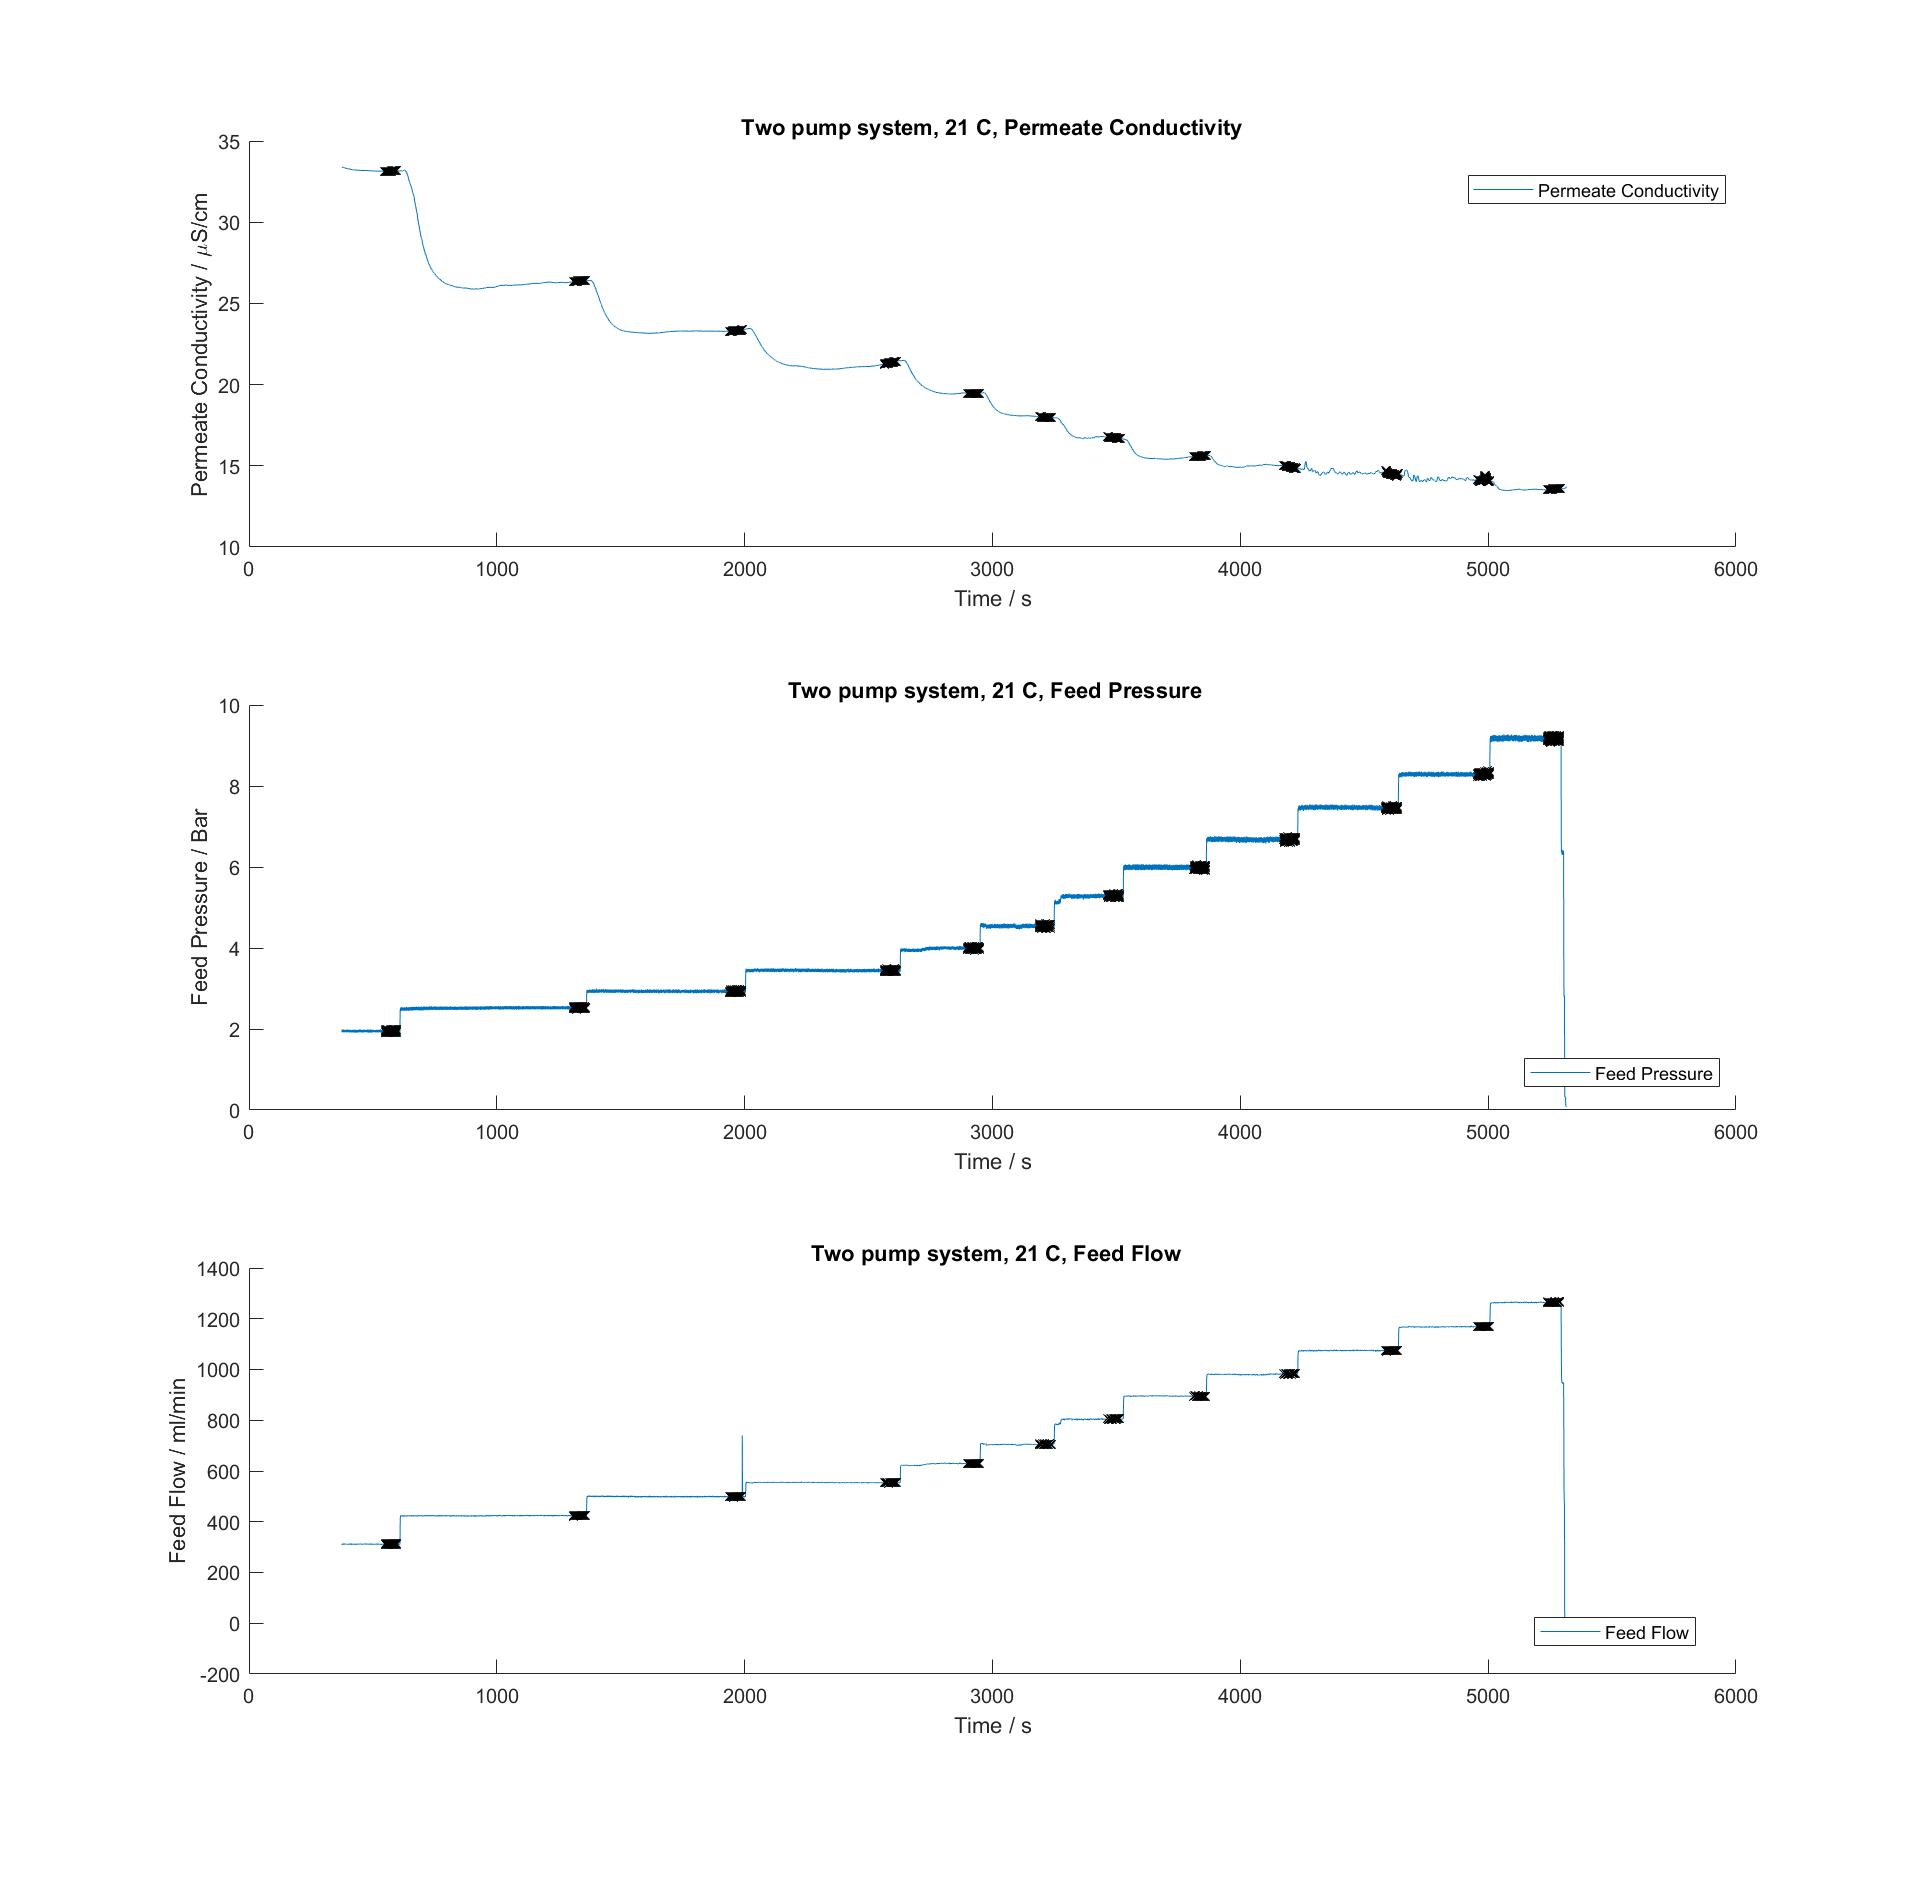
\includegraphics[width=1.1\textwidth]{FeedPumpIncrease21}
    \caption{Connections Pressure sensors}
    \label{fig:PressConn}
\end{figure}


\begin{figure}[H]
    \centering
    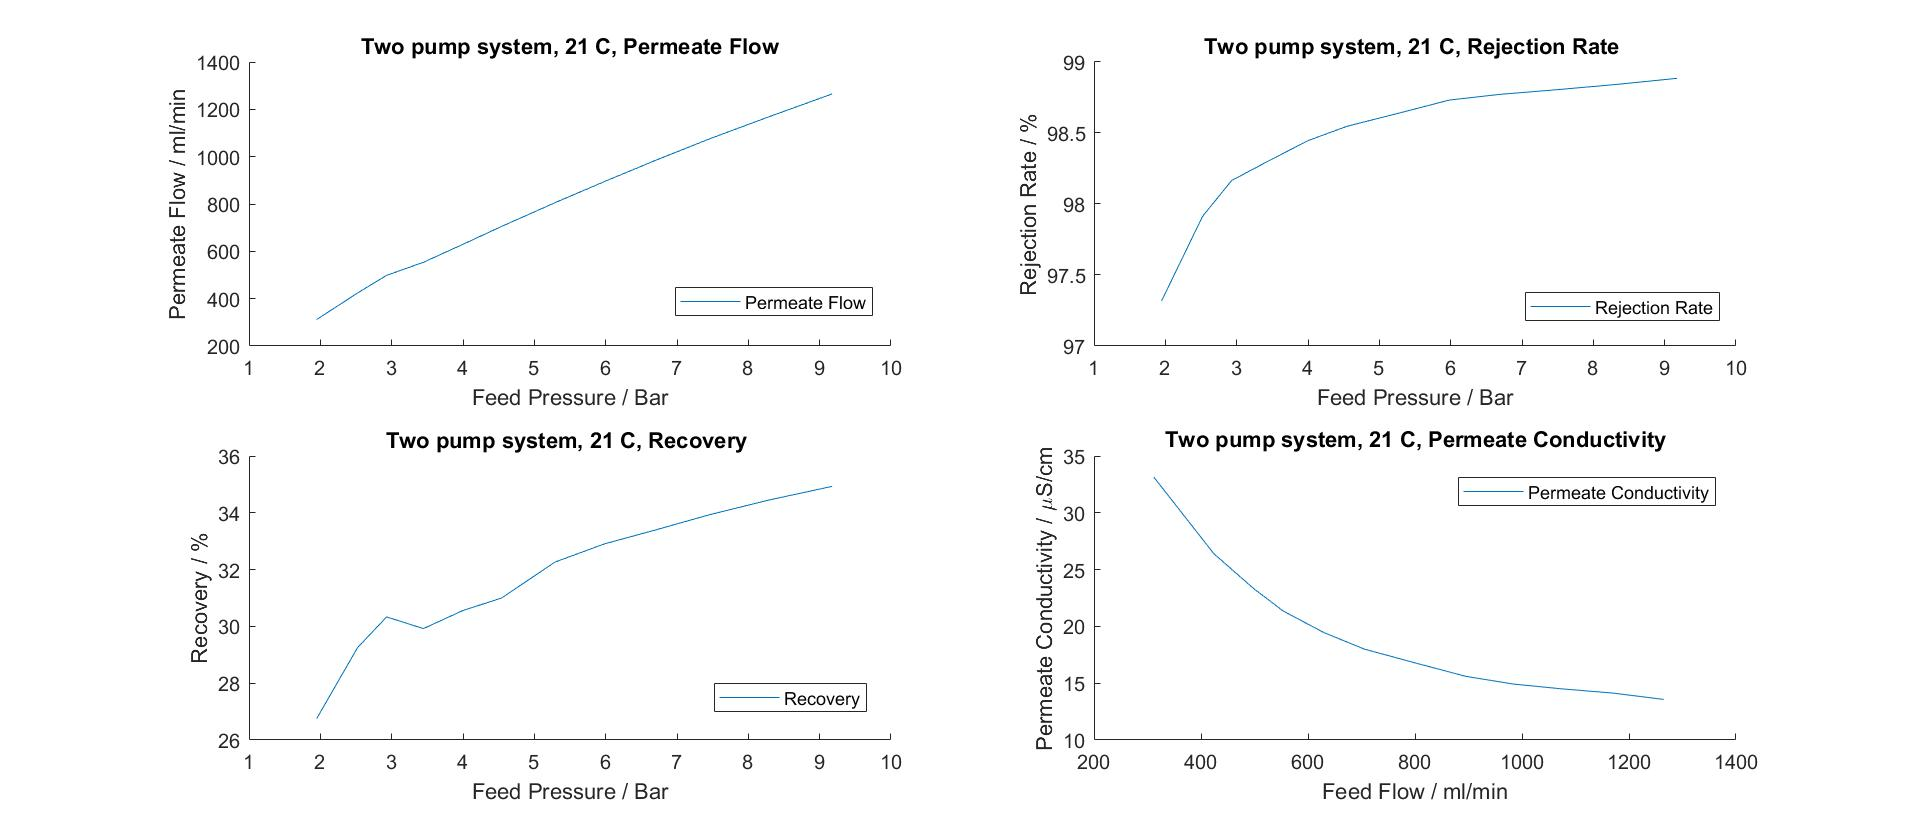
\includegraphics[width=1.1\textwidth]{FeedPumpIncrease21Key}
    \caption{Connections Pressure sensors}
    \label{fig:PressConn}
\end{figure}

30


\begin{figure}[H]
    \centering
    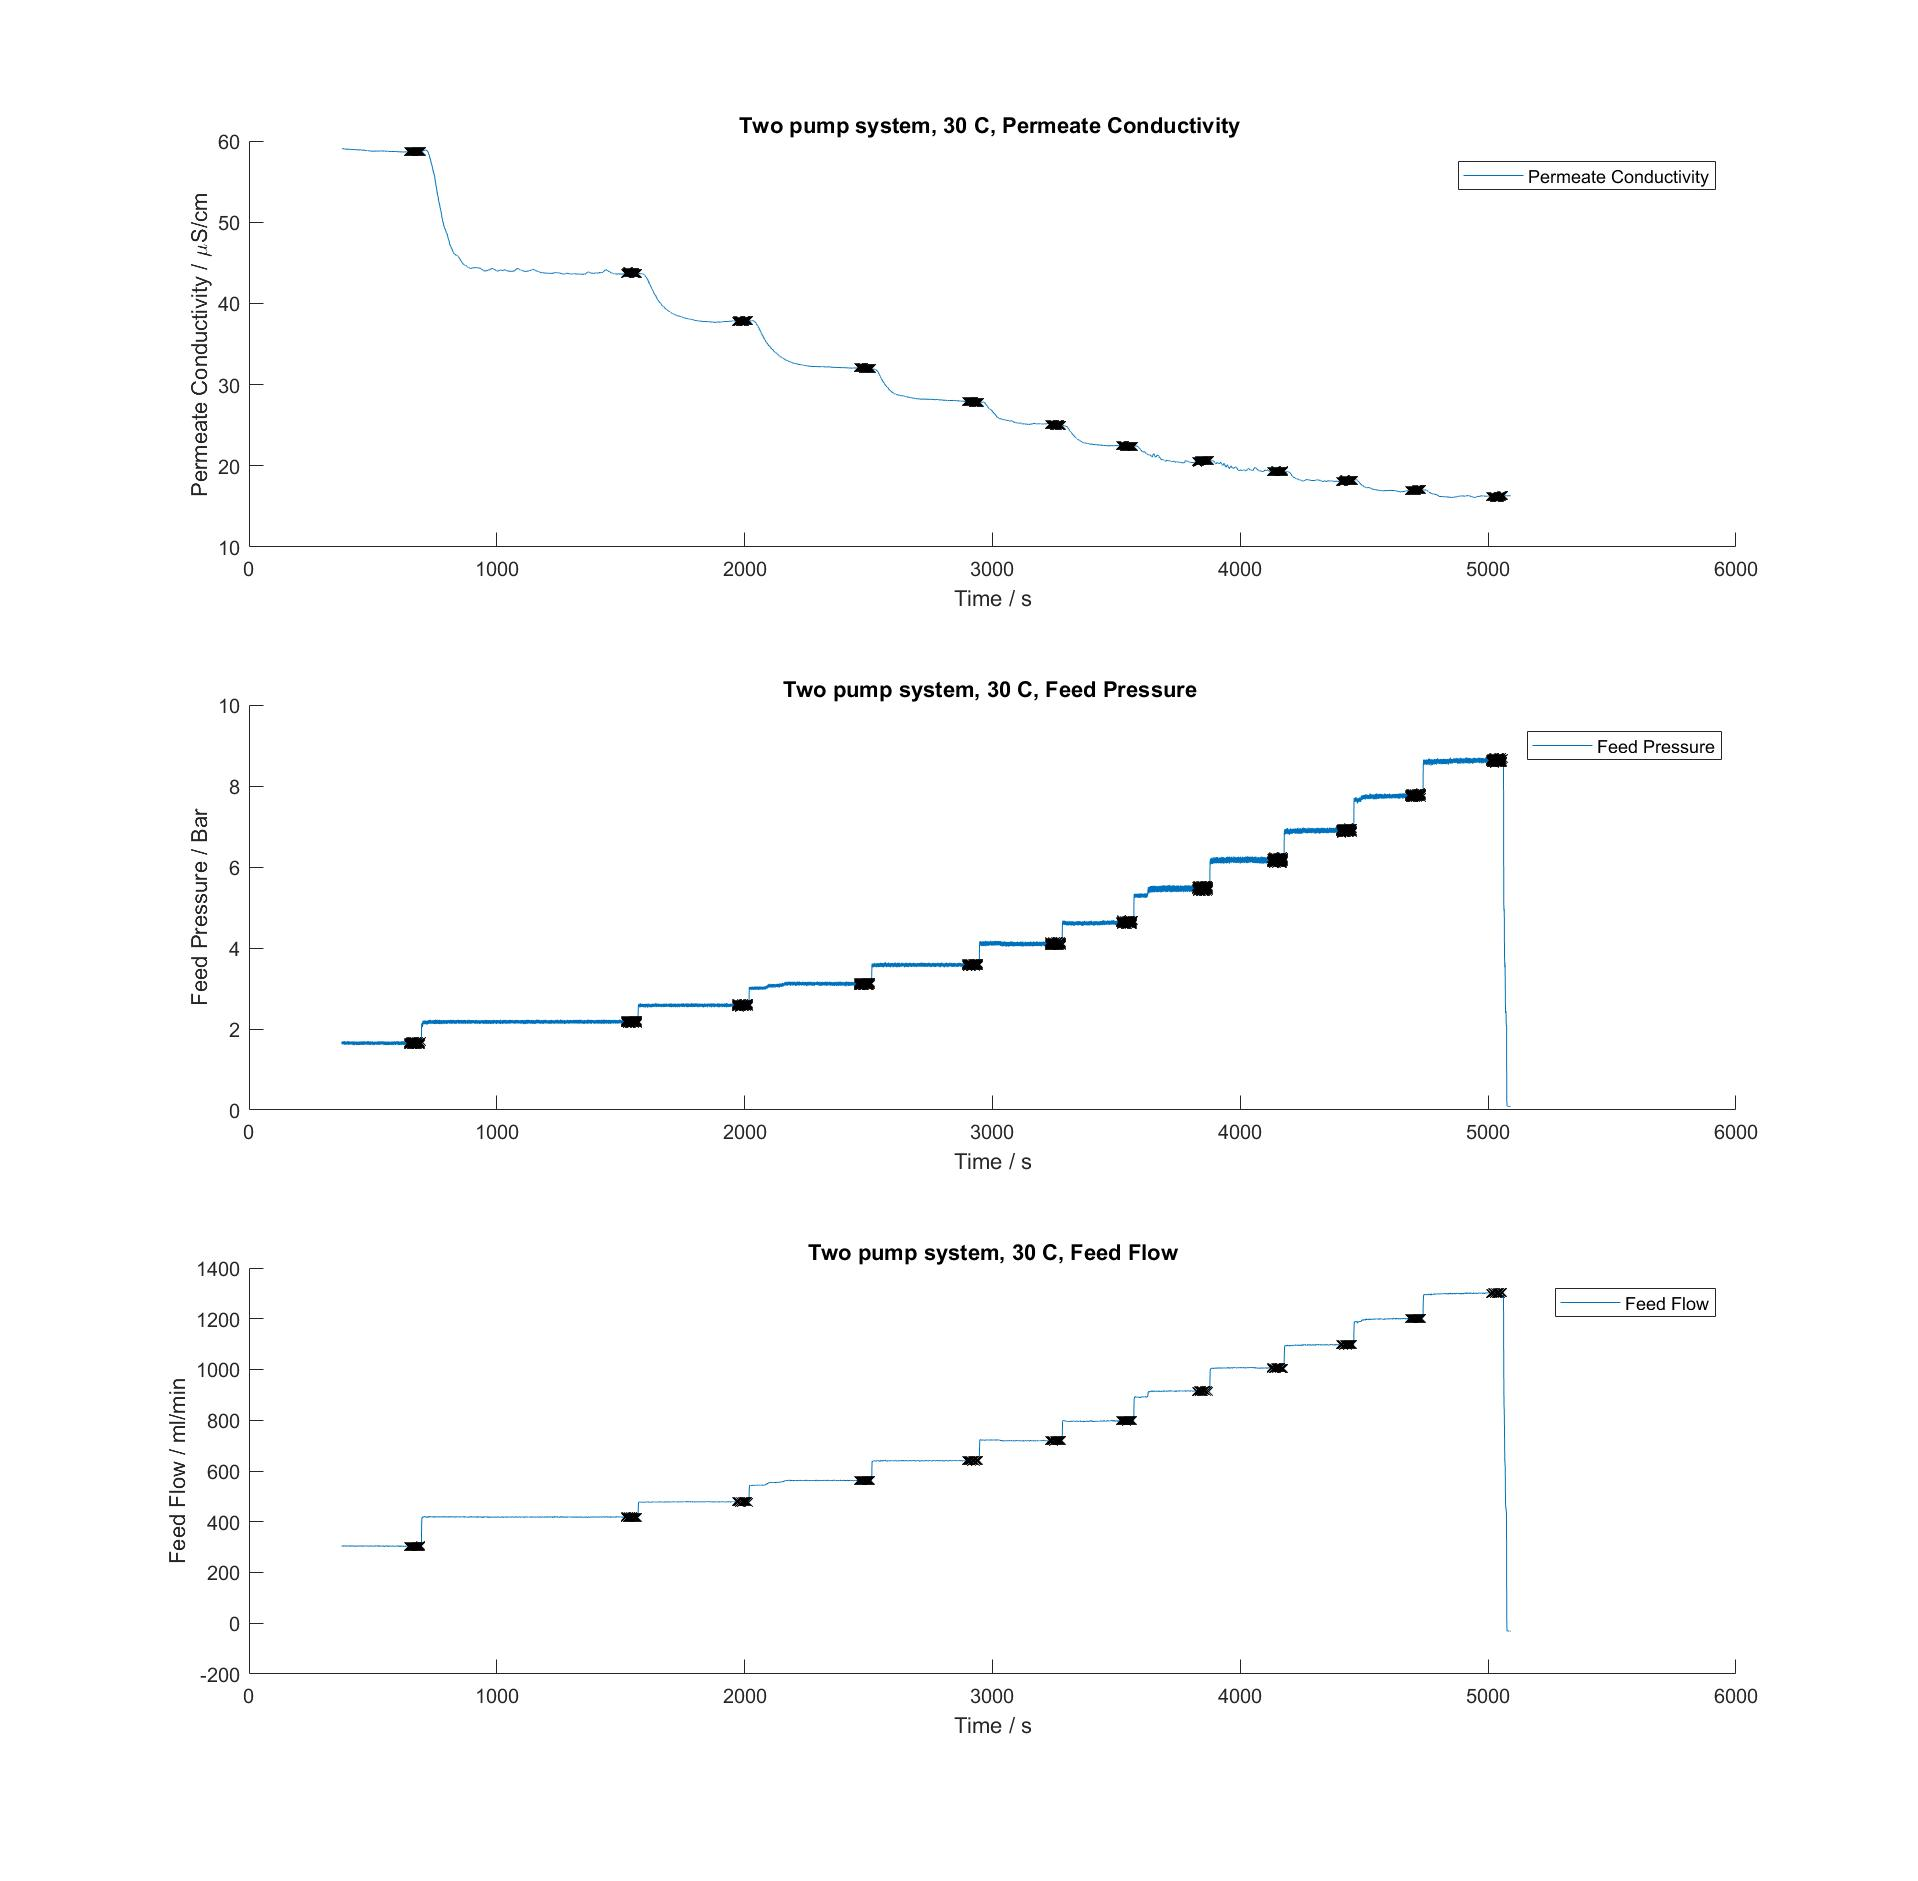
\includegraphics[width=1.1\textwidth]{FeedPumpIncrease30}
    \caption{Connections Pressure sensors}
    \label{fig:PressConn}
\end{figure}


\begin{figure}[H]
    \centering
    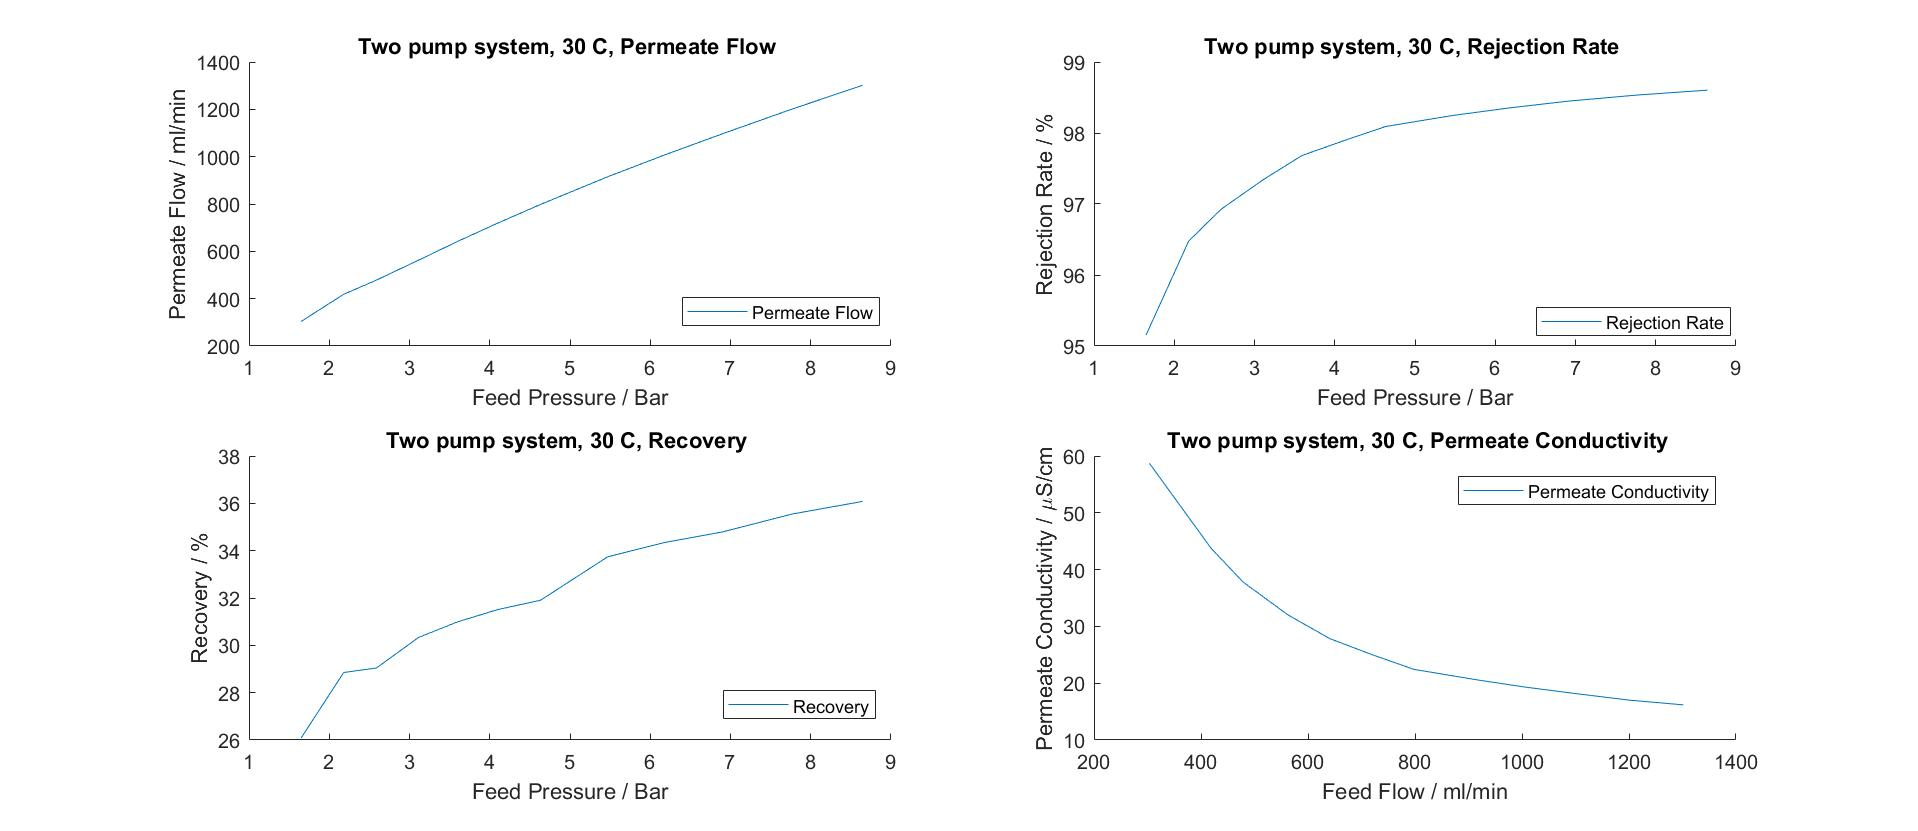
\includegraphics[width=1.1\textwidth]{FeedPumpIncrease30Key}
    \caption{Connections Pressure sensors}
    \label{fig:PressConn}
\end{figure}

40


\begin{figure}[H]
    \centering
    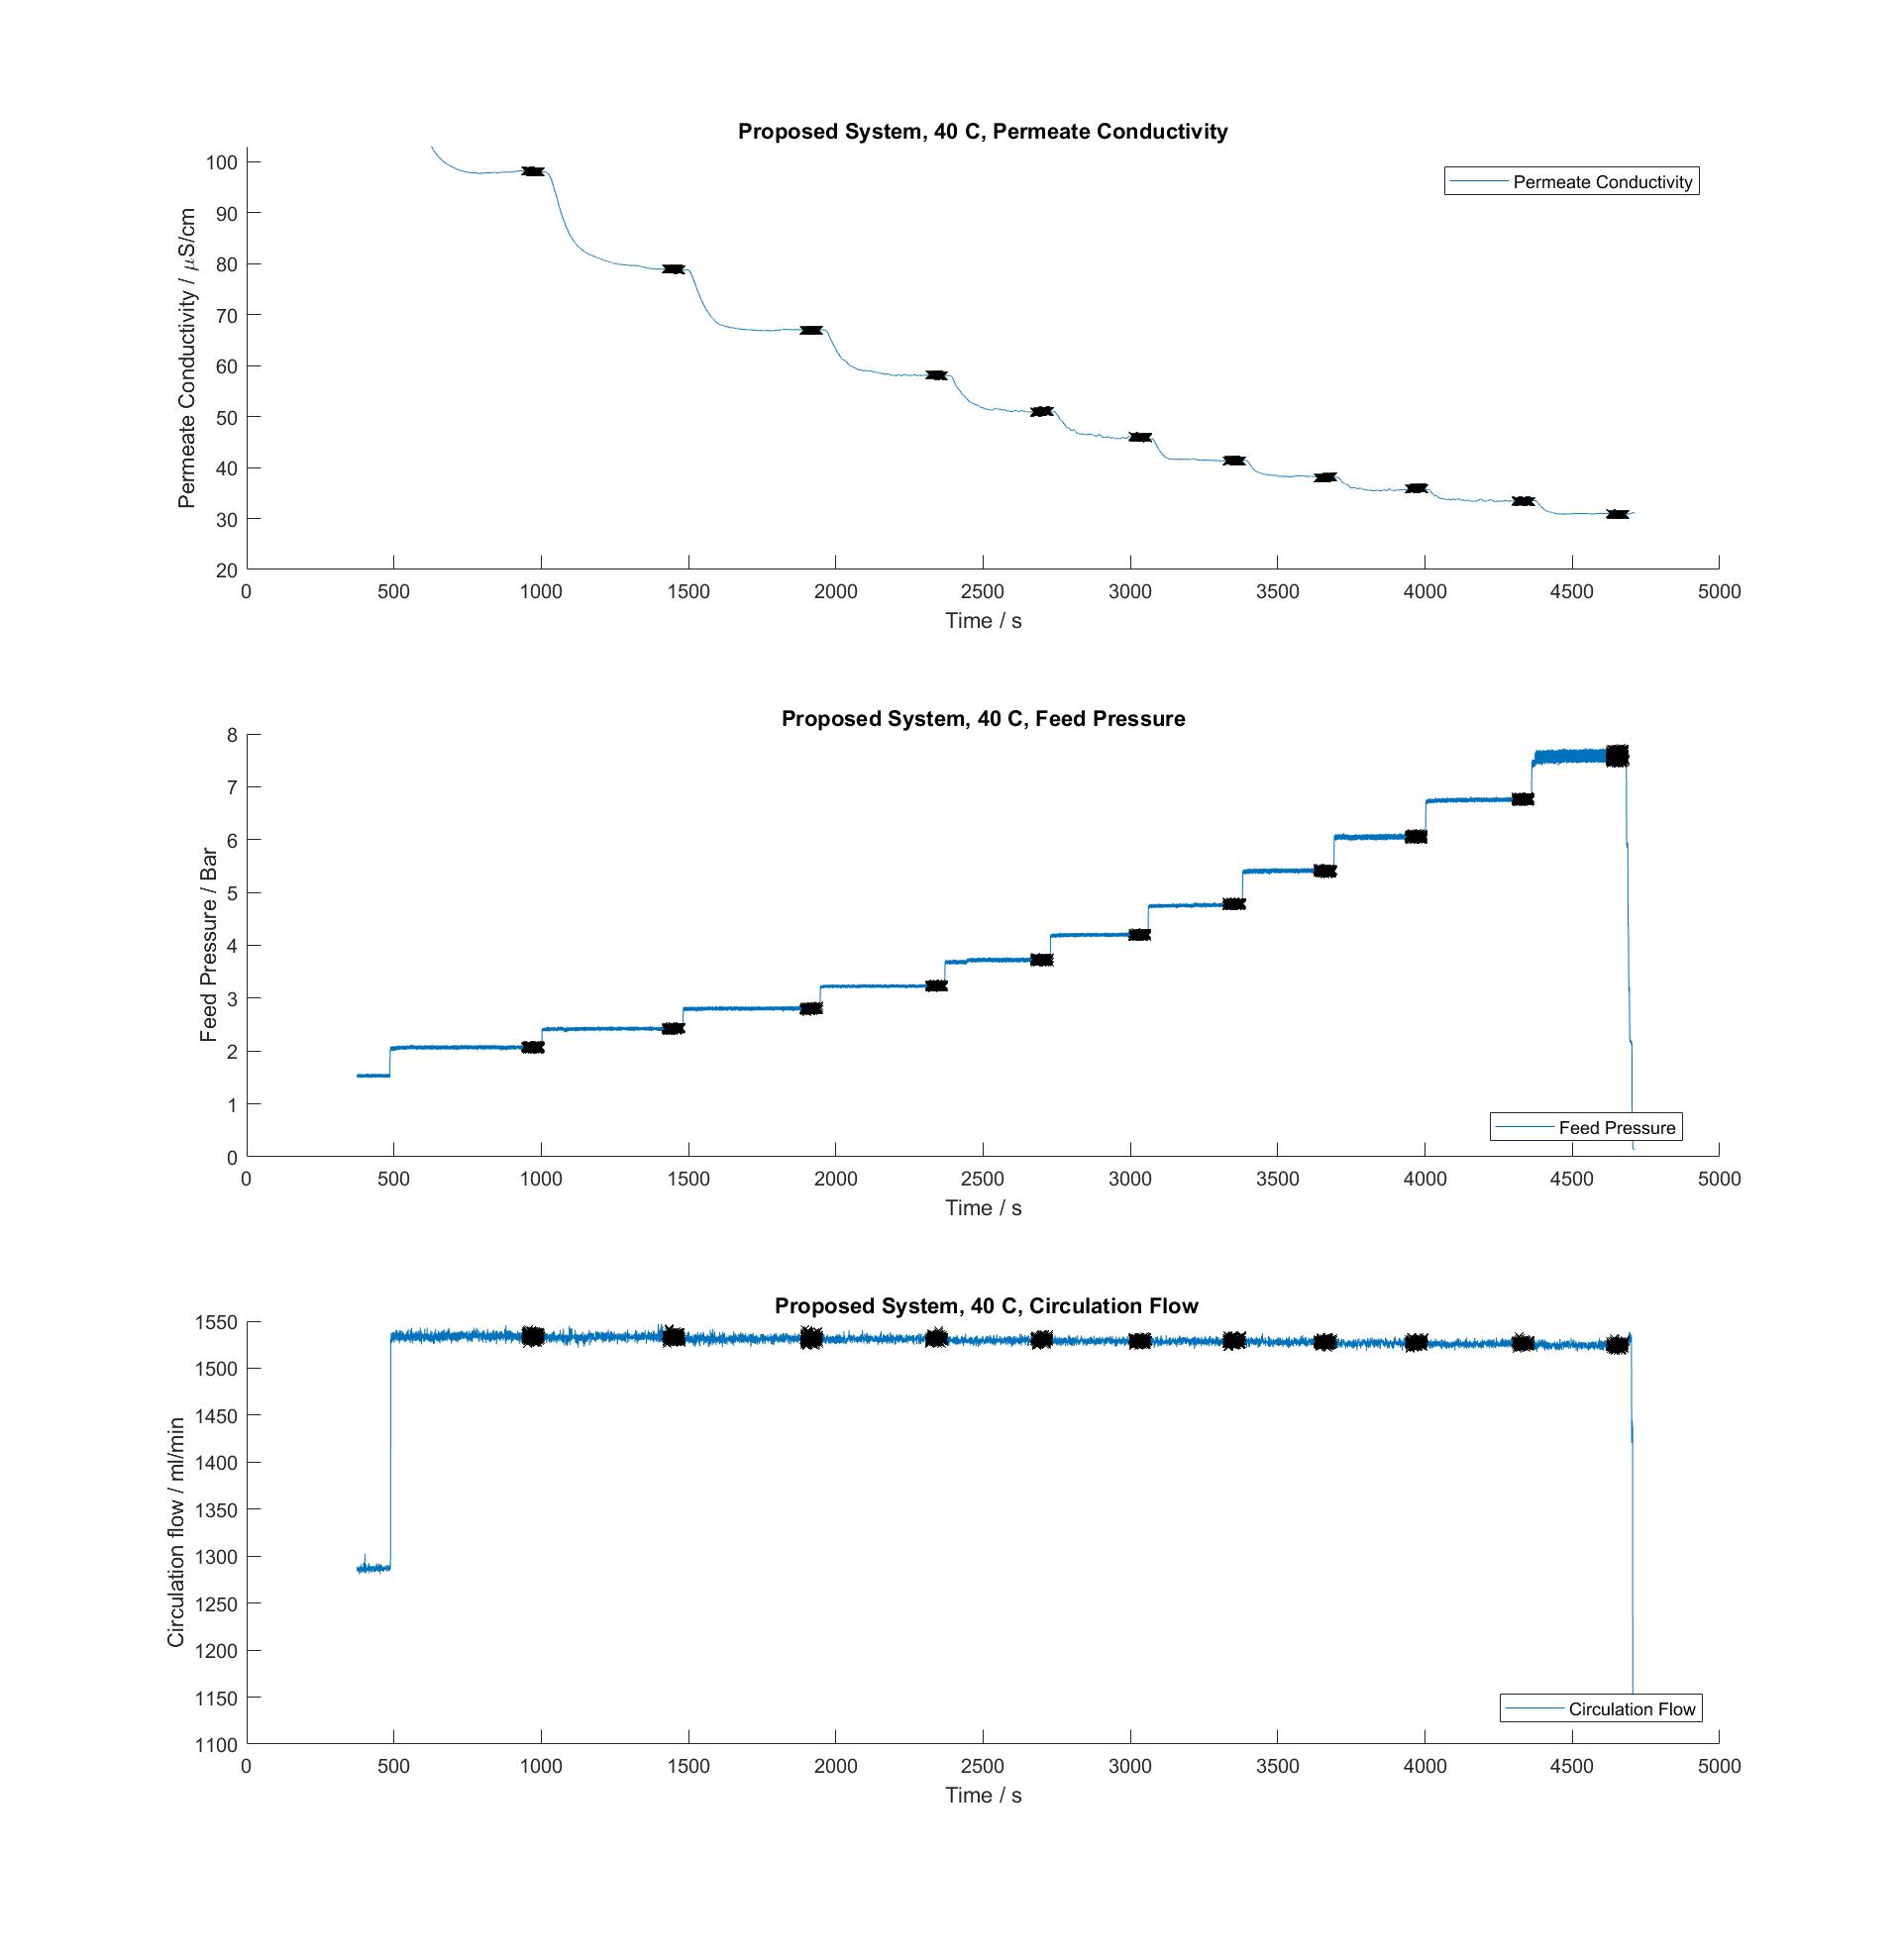
\includegraphics[width=1.1\textwidth]{FeedPumpIncrease40}
    \caption{Connections Pressure sensors}
    \label{fig:PressConn}
\end{figure}


\begin{figure}[H]
    \centering
    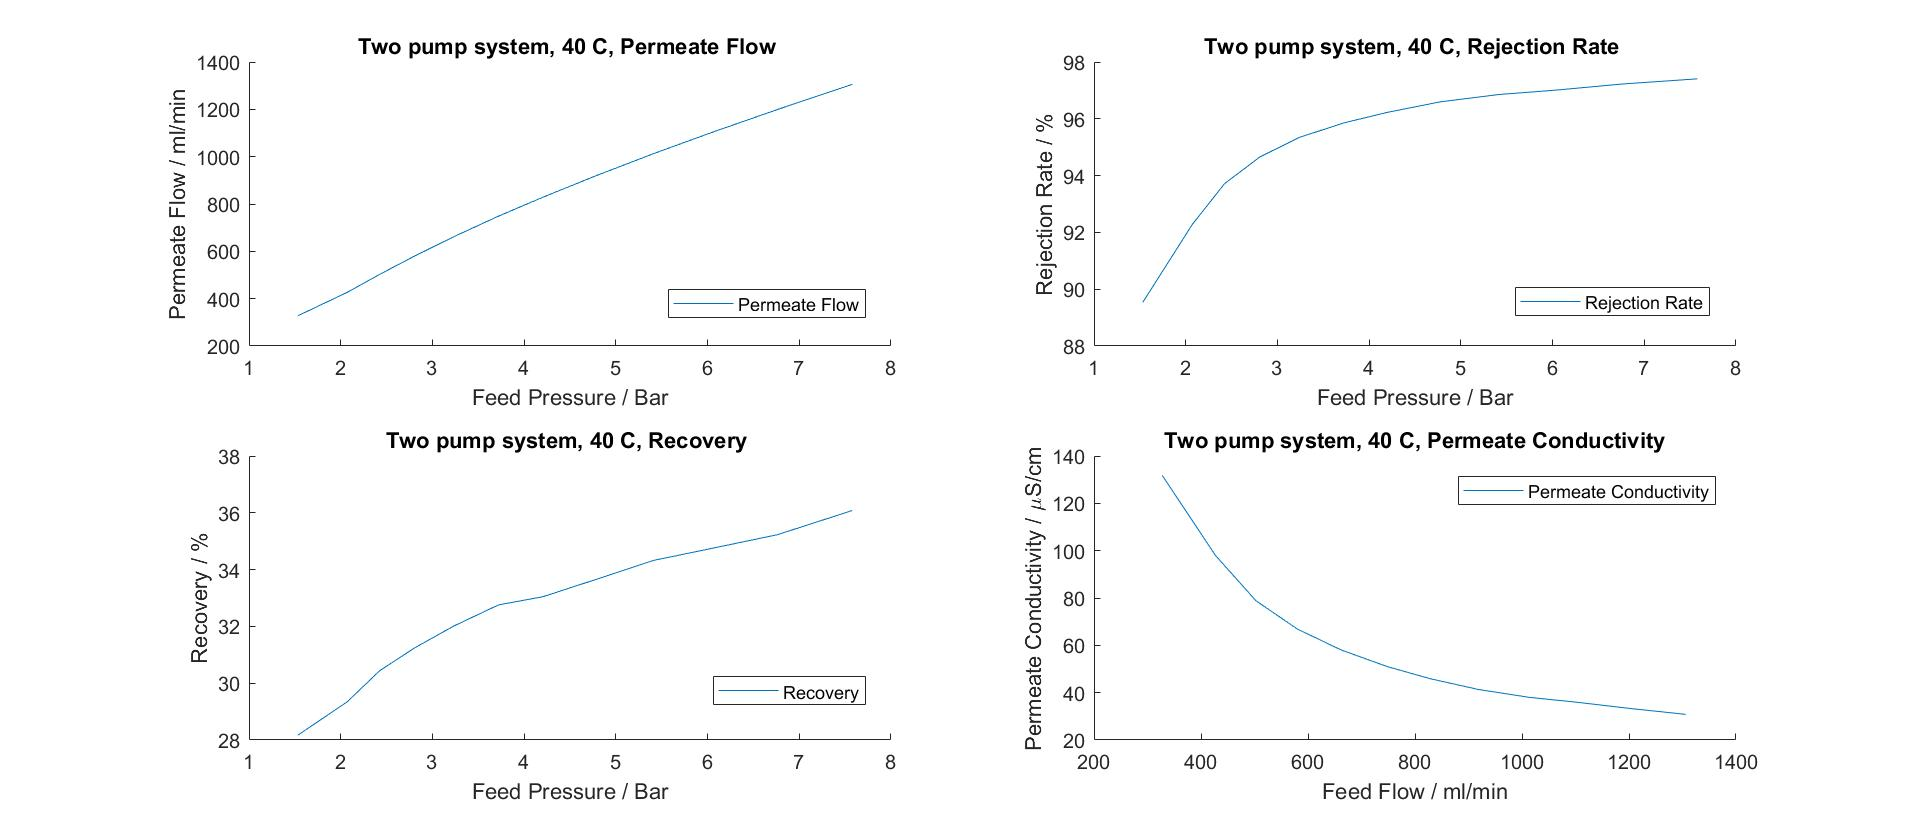
\includegraphics[width=1.1\textwidth]{FeedPumpIncrease40Key}
    \caption{Connections Pressure sensors}
    \label{fig:PressConn}
\end{figure}

Recovery Increase

\begin{figure}[H]
    \centering
    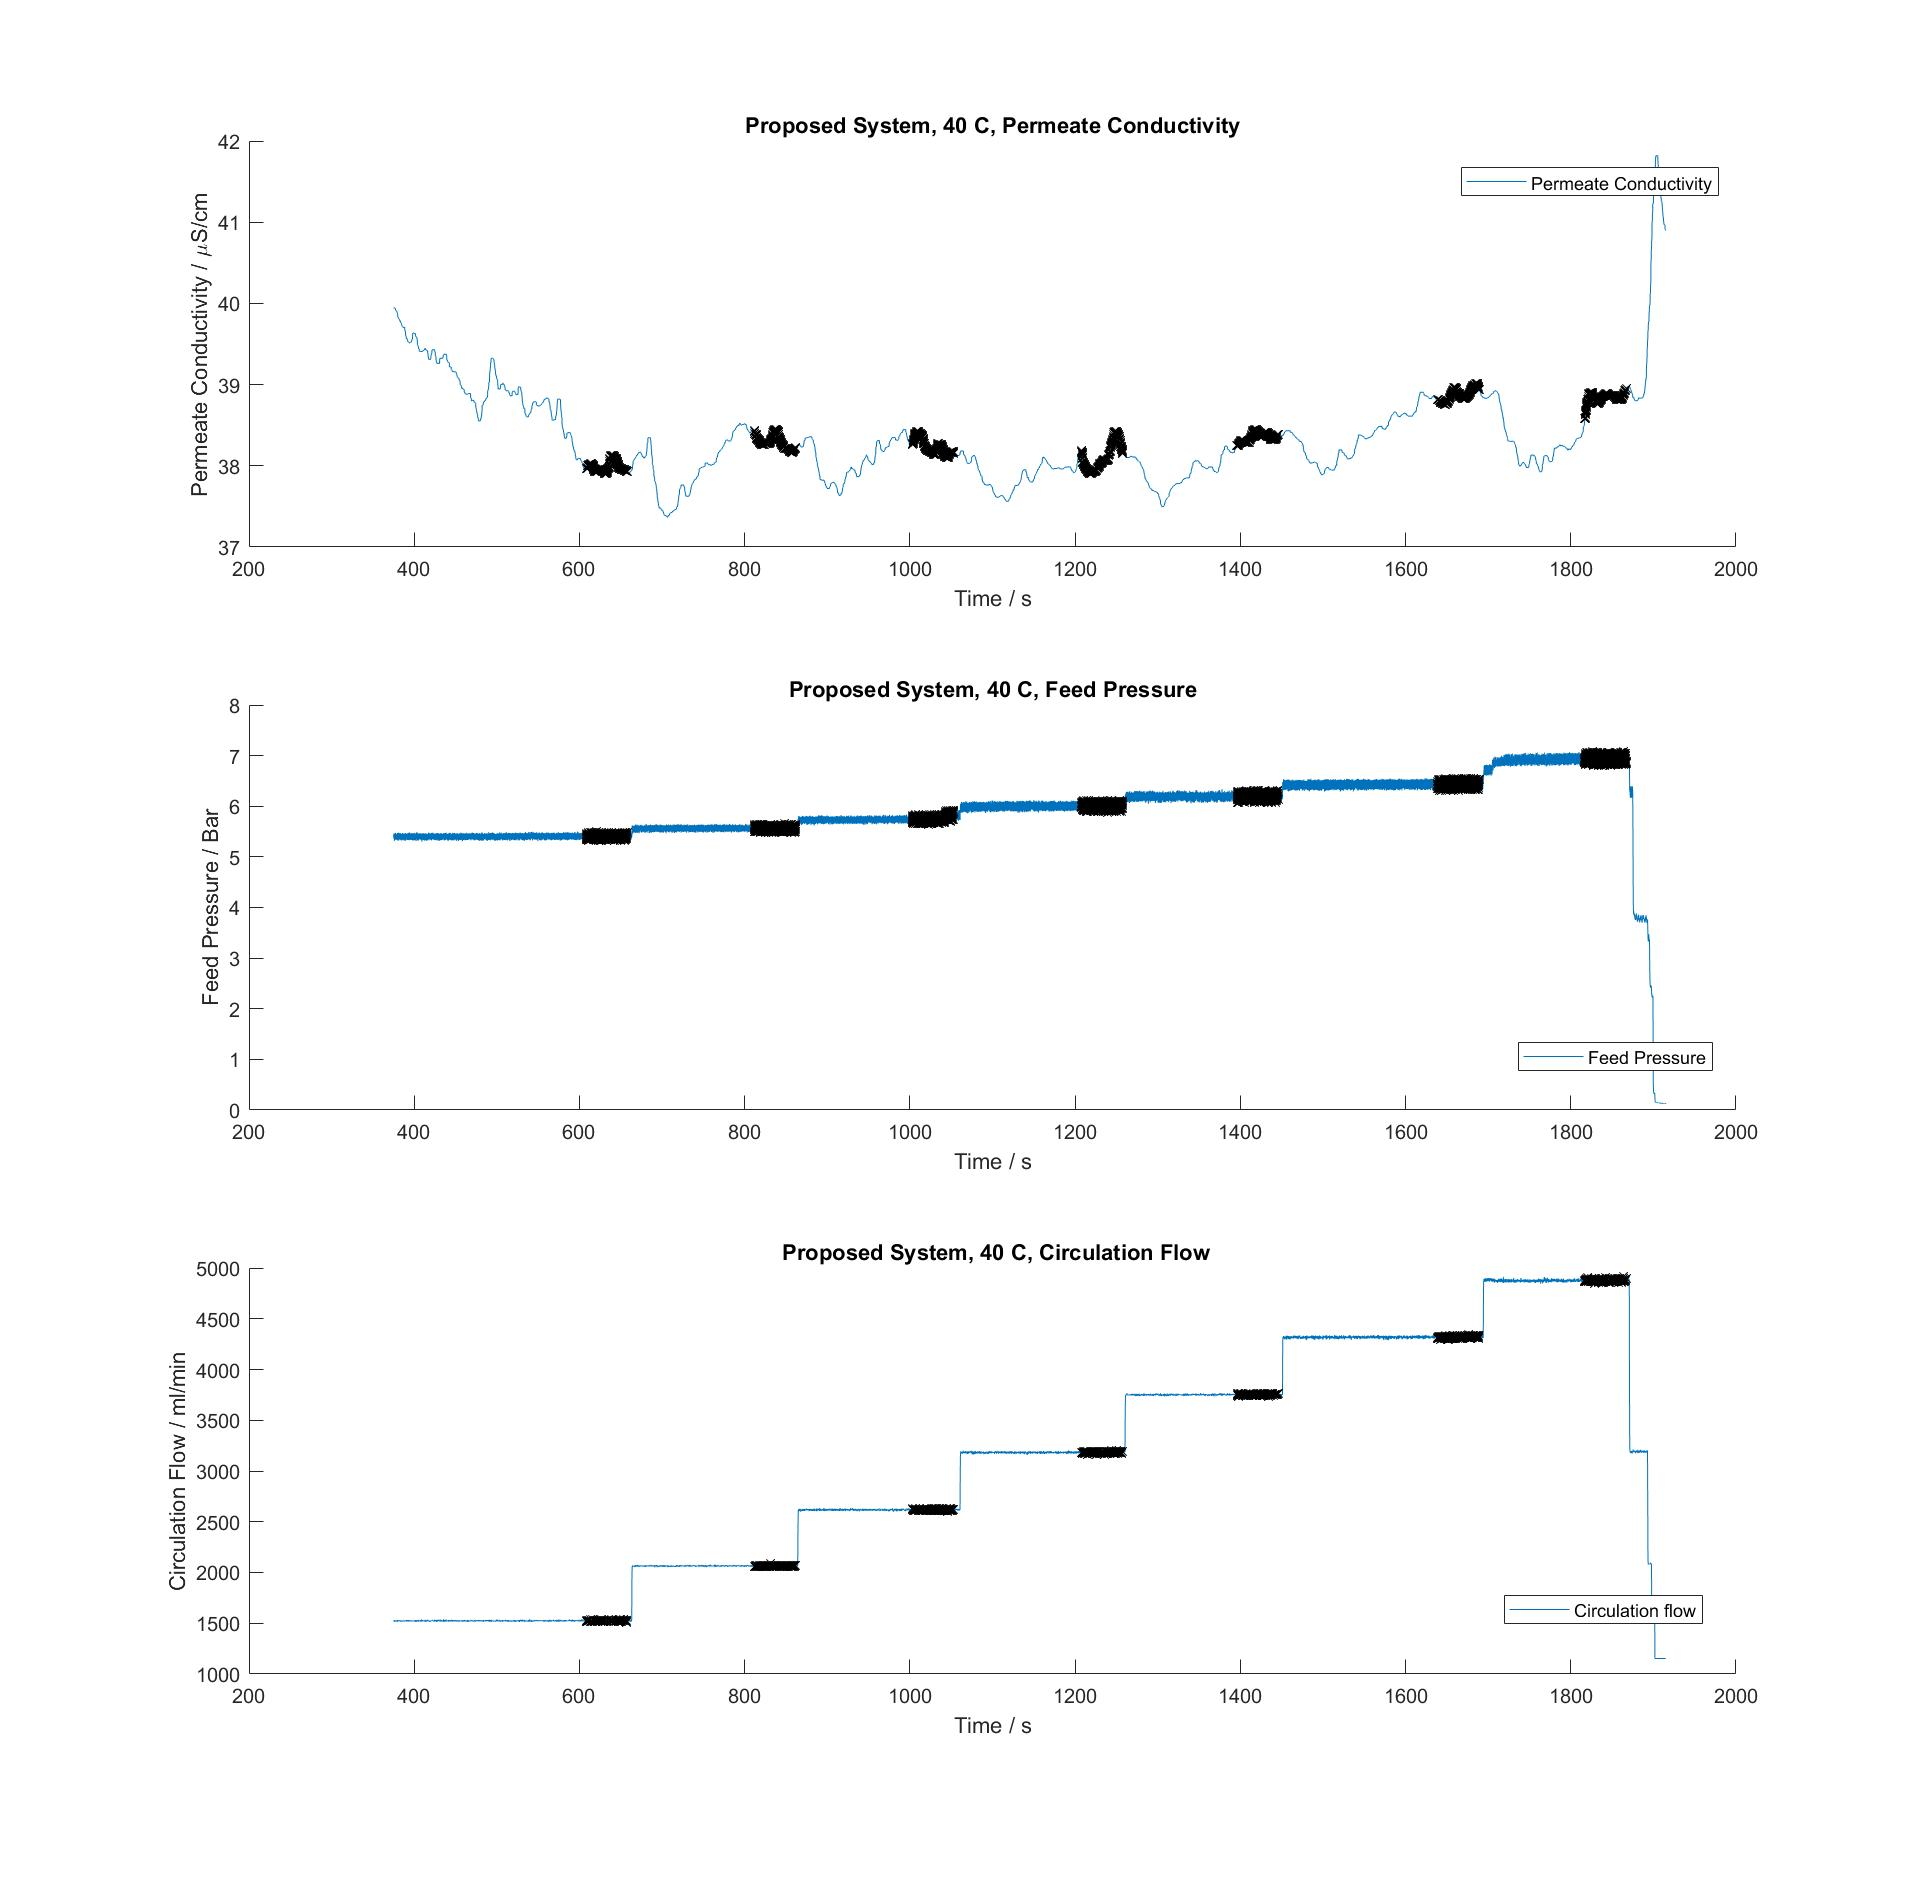
\includegraphics[width=1.1\textwidth]{RecIncrease40}
    \caption{Connections Pressure sensors}
    \label{fig:PressConn}
\end{figure}

\begin{figure}[H]
    \centering
    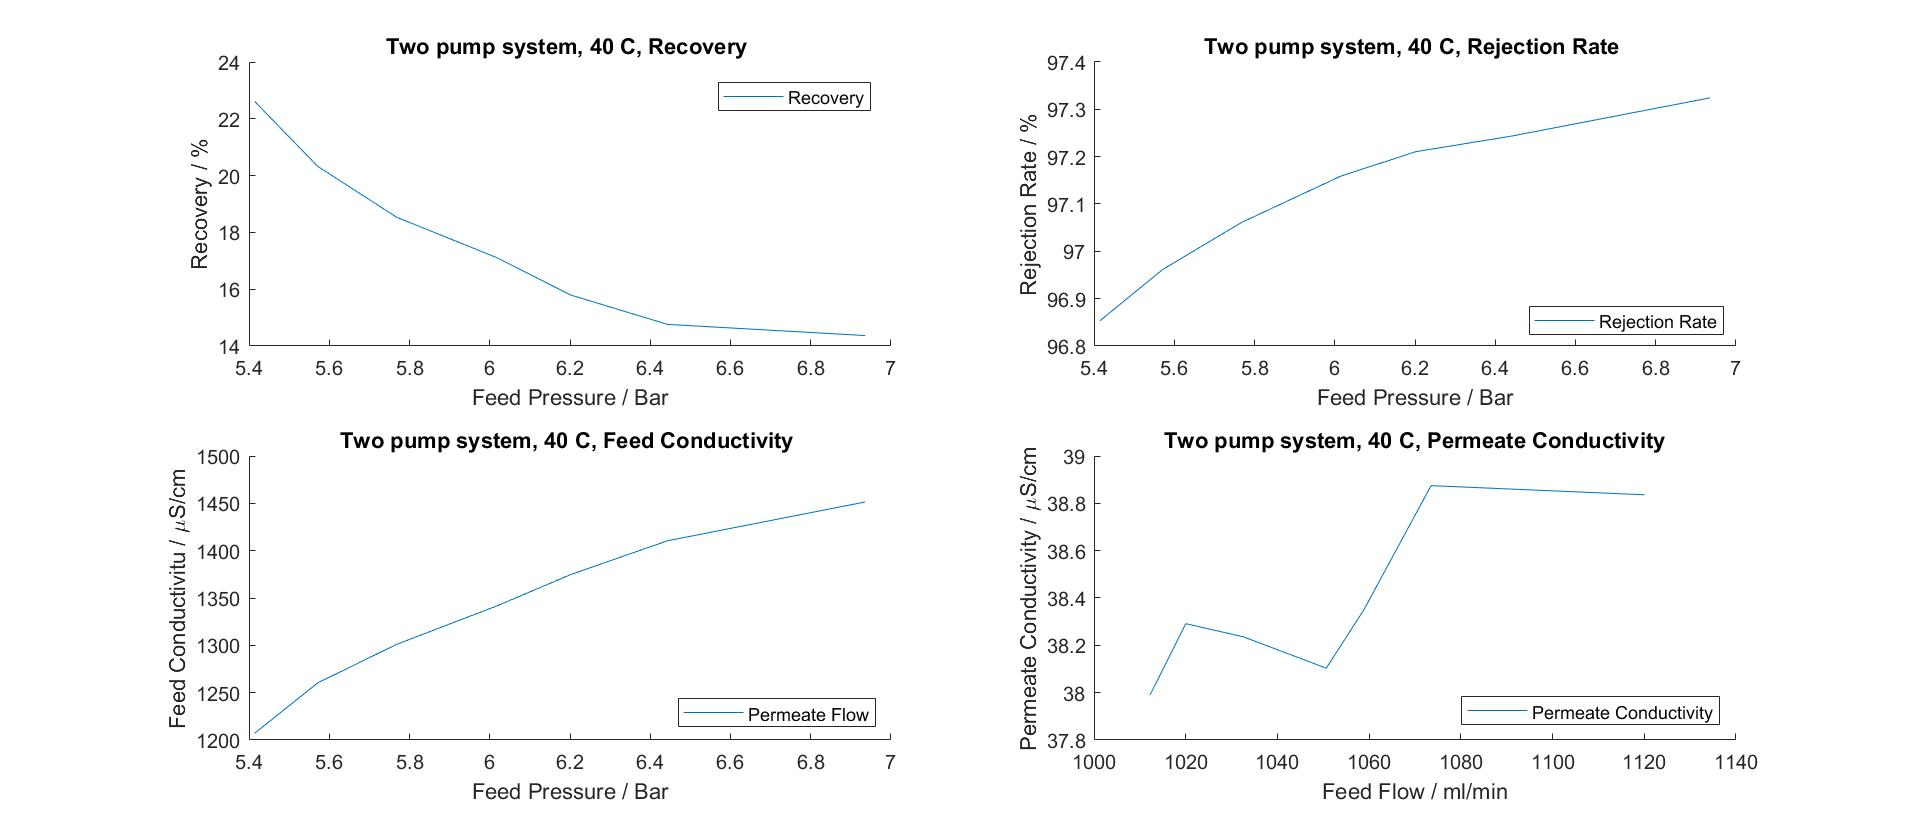
\includegraphics[width=1.1\textwidth]{RecIncrease40Key}
    \caption{Connections Pressure sensors}
    \label{fig:PressConn}
\end{figure}








\section{Modeling}
A physical model of the membrane were made and the given results can be seen in: 

\section{Implementation Test Rig}


\subsection{Connections}
In Figure (\ref{fig:PressConn}-\ref{fig:PumpConn}) all connections in the test rig is displayed.


\begin{figure}[h]
    \centering
    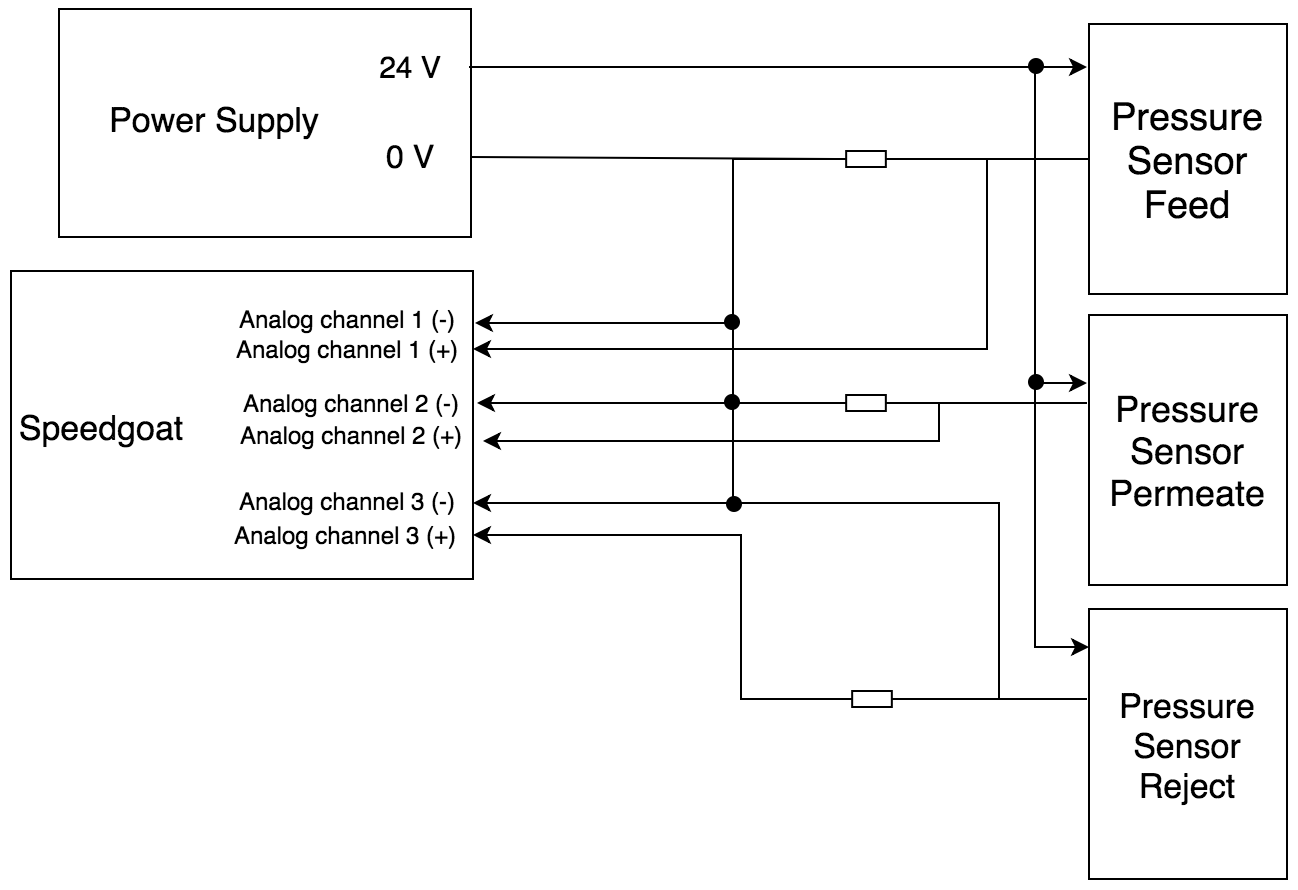
\includegraphics[width=0.7\textwidth]{PressConn}
    \caption{Connections Pressure sensors}
    \label{fig:PressConn}
\end{figure}

\begin{figure}[h]
    \centering
    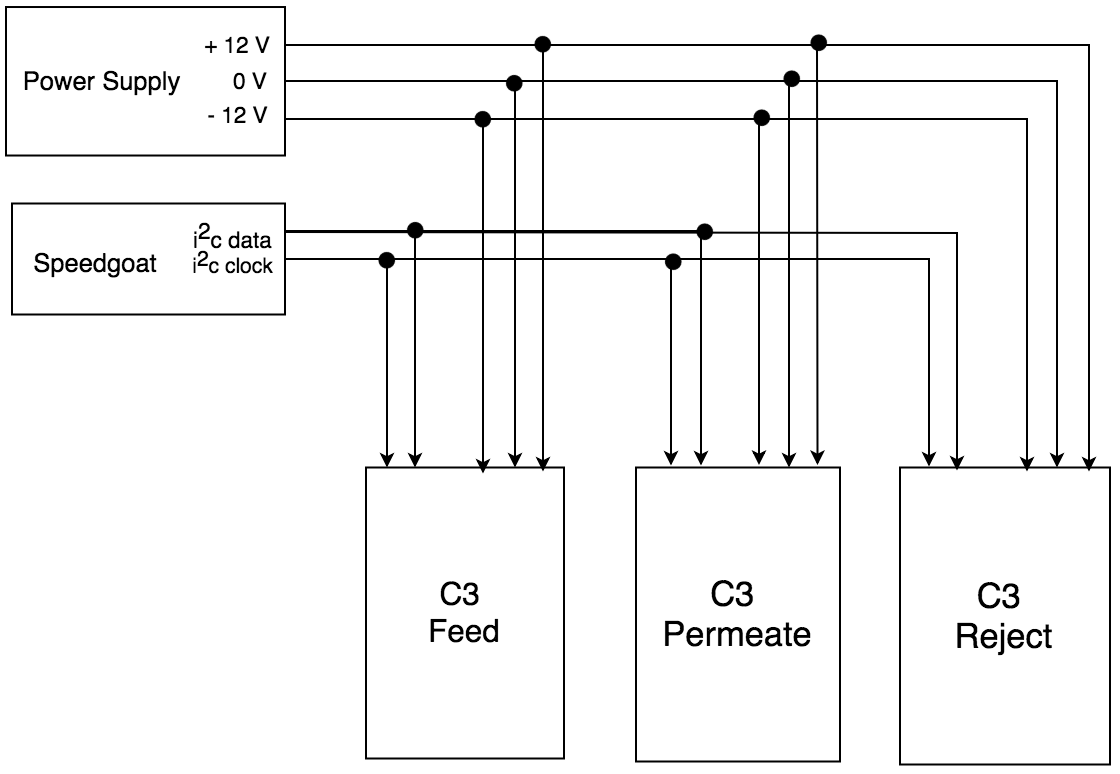
\includegraphics[width=0.7\textwidth]{C3Conn}
    \caption{Connections measurement blocks, C3}
    \label{fig:C3Conn}
\end{figure}

\begin{figure}[h]
    \centering
    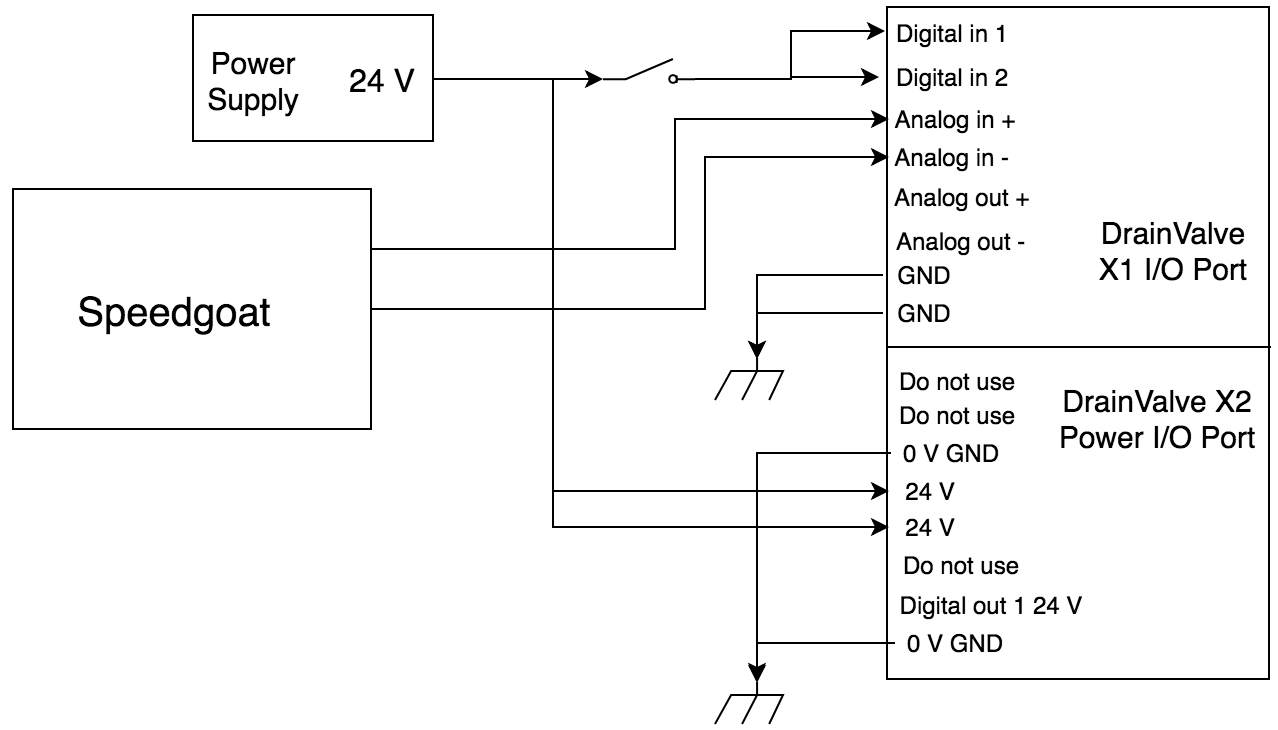
\includegraphics[width=0.7\textwidth]{ValveConn}
    \caption{Connections Drain Valve}
    \label{fig:ValveConn}
\end{figure}

\begin{figure}[h]
    \centering
    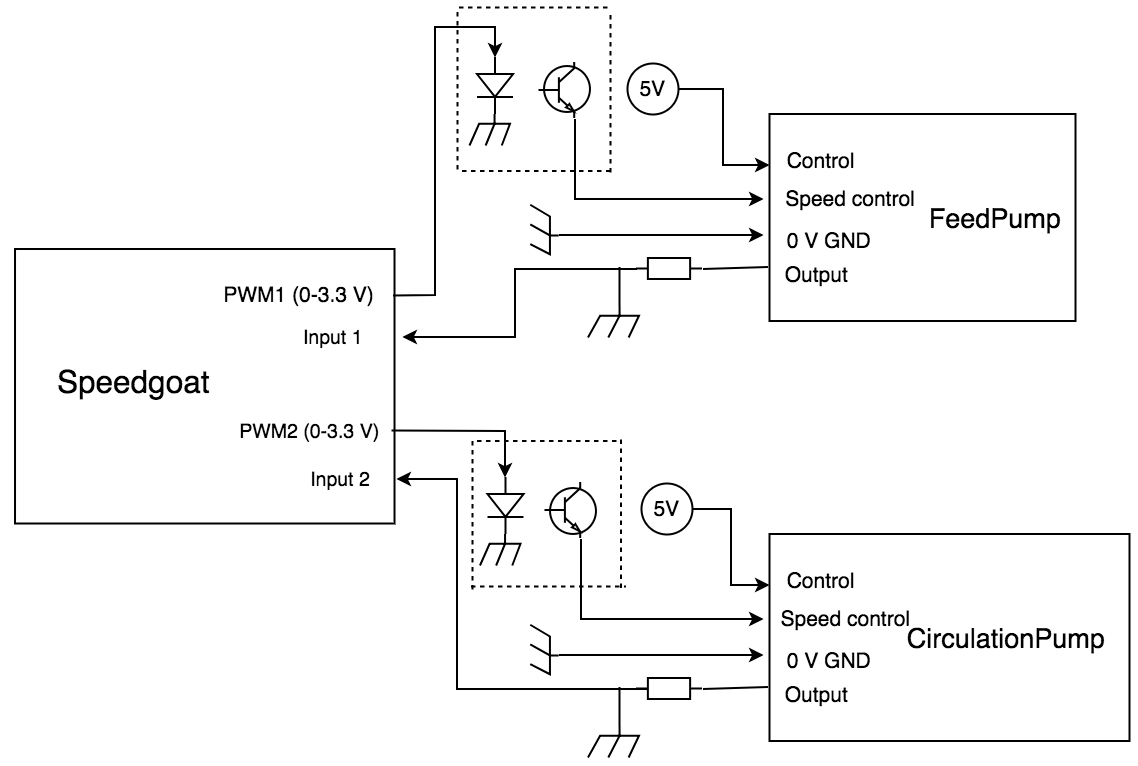
\includegraphics[width=0.7\textwidth]{PumpConn}
    \caption{Connections pumps}
    \label{fig:PumpConn}
\end{figure}


\section{Mapping}
\begin{figure}[h]
    \centering
    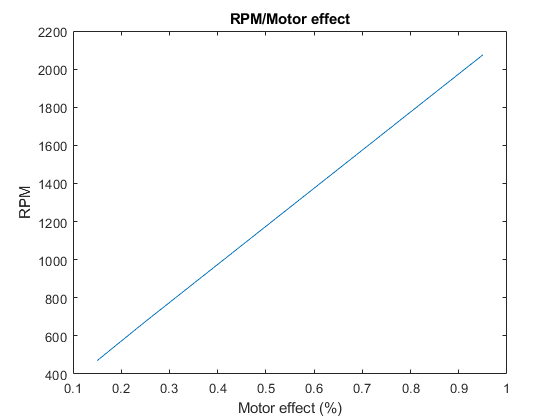
\includegraphics[width=0.7\textwidth]{RPM.png}
    \caption{RPM Pumps}
    \label{fig:RPM}
\end{figure}


\begin{figure}[h]
    \centering
    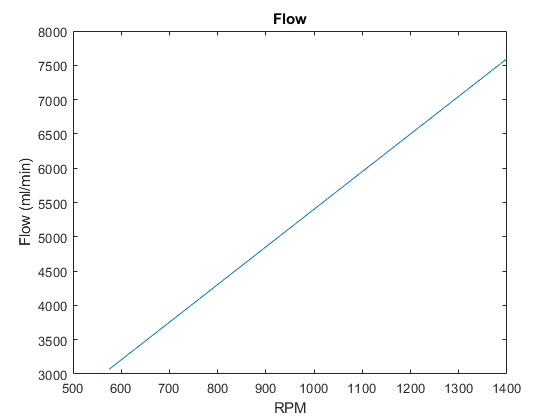
\includegraphics[width=0.7\textwidth]{Flow.png}
    \caption{Flowrate}
    \label{fig:Flowrate}
\end{figure}


\section{Design of control algorithms}

\begin{figure}[h]
    \centering
    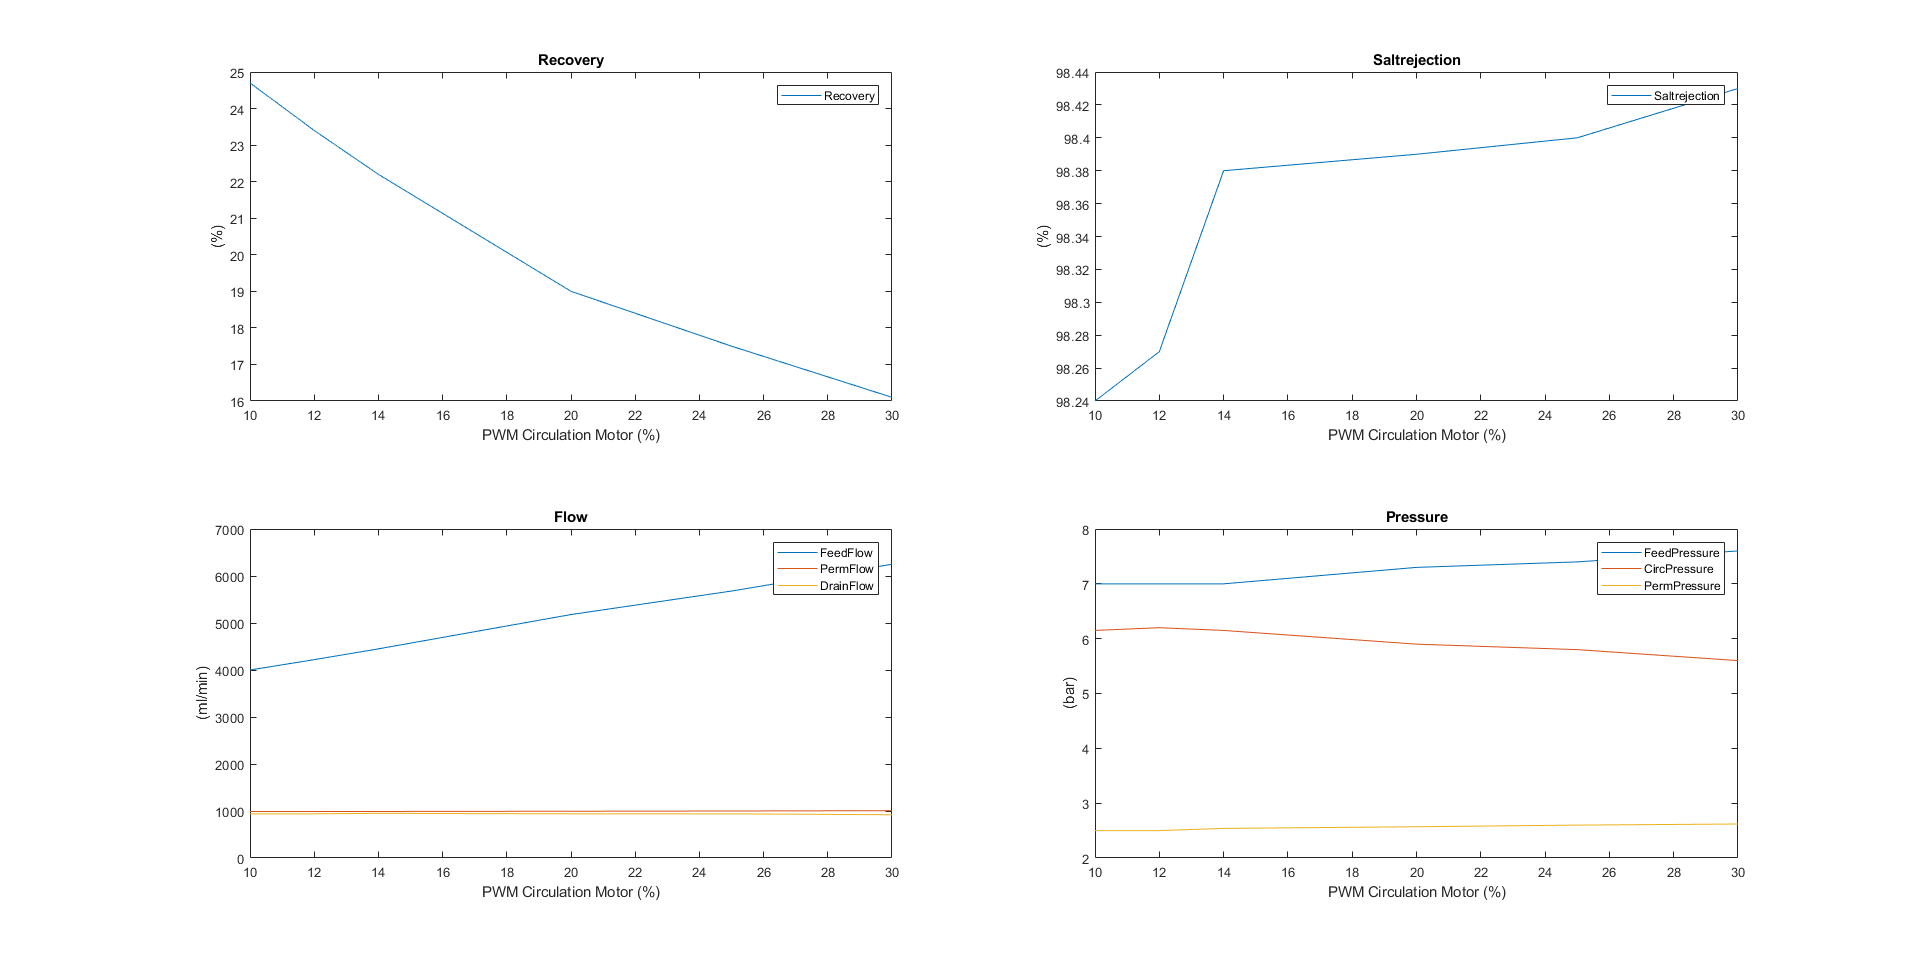
\includegraphics[width=1.65\textwidth, angle = 270]{PreTestReg1.png}
    \caption{Tests with recycle pump as changing parameter}
    \label{fig:PreTestReg1}
\end{figure}

\begin{figure}[h]
    \centering 
    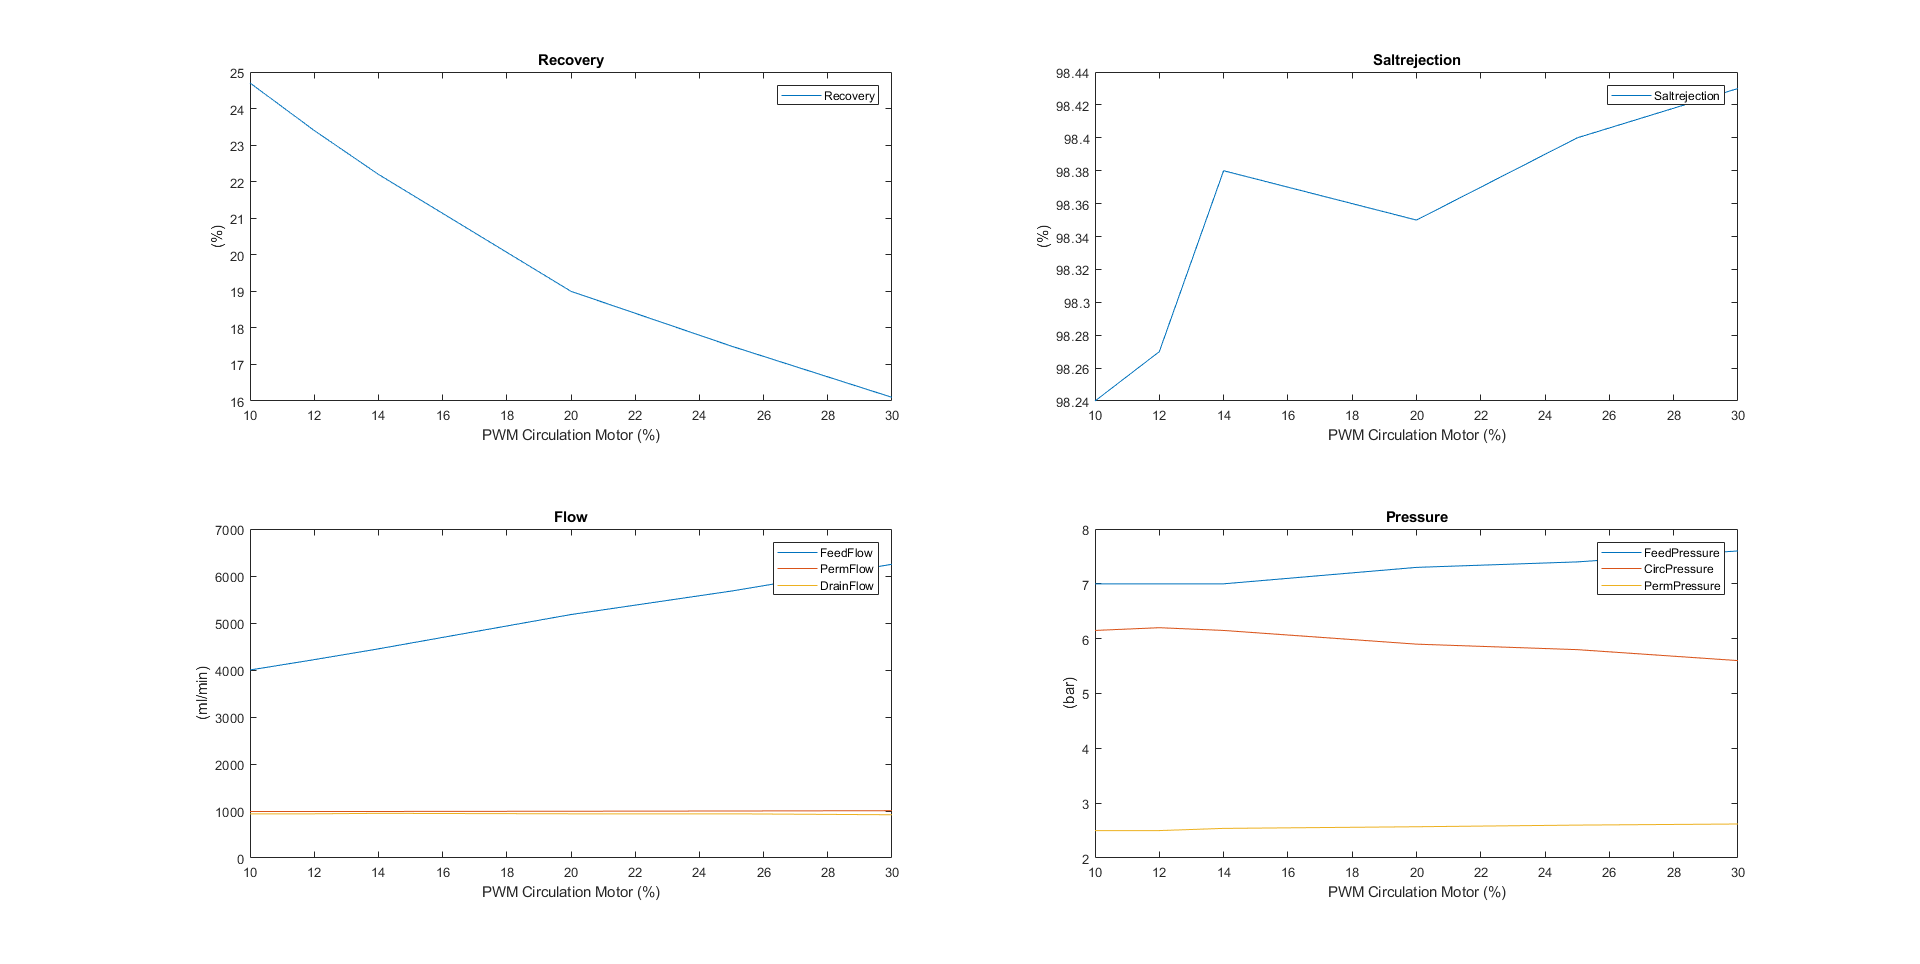
\includegraphics[width=1.65\textwidth, angle=270]{PreTestReg3.png}
    \caption{Tests with inlet pump as changing parameter}
    \label{fig:PreTestReg3}
\end{figure}





FIGURES AND PLOTS FROM SIMSCAPE


\section{Control simulations}




\section{Improvements}
